% Inbuilt themes in beamer
\documentclass{beamer}


%Defining some colours
\definecolor{darkred}{rgb}{0.8,0,0}

% Theme choice: there a number of preset themes to choose from
% Play around with them, Cambridge is nice for first pres
%\usetheme{Szeged}
\usetheme{CambridgeUS} %setting the main theme
\usecolortheme{whale} % setting colour theme
\usefonttheme{professionalfonts} %font theme
\useinnertheme[shadow=true]{rounded}
%\useoutertheme{} %outer theme

%\setbeamertemplate{footline} %Remove footer line in all slides
\setbeamertemplate{navigation symbols}{} %removes navigation symbols
\setbeamertemplate{footline}[page number] %removes footer line, keeps pg#
\setbeamertemplate{caption}{\insertcaption} 


%Setting colours for boxes and captions
\setbeamercolor{block title}{bg=blue!30, fg=black}
\setbeamercolor{block body}{bg=blue!10}
\setbeamercolor{frametitle}{fg=black}

%%%FOR VIDEOS
\usepackage{media9}
\usepackage{multimedia}
\usepackage{graphicx}
% For the Flowchart
%\usepackage{tikz}
%\usetikzlibrary{shapes.geometric, arrows}
%\tikzstyle{startstop} = [rectangle, rounded corners, minimum width=3cm, minimum height=1cm,text centered, draw=black, fill=blue!30]
%\tikzstyle{process} = [rectangle, minimum width=3cm, minimum height=1cm, text centered, draw=black, fill=orange!30]
%\tikzstyle{decision} = [diamond, minimum width=3cm, minimum height=1cm, text centered, draw=black, fill=green!30]
%\tikzstyle{arrow} = [thick,->,>=stealth]

%%% For the Timeline
\usepackage{xcolor}
\usepackage{tikz} \usetikzlibrary{calc, arrows.meta, intersections, patterns, positioning, shapes.misc, fadings, through,decorations.pathreplacing}

\definecolor{ColorOne}{rgb}{0.0,0.5,1.0} %Lightblue
\definecolor{ColorTwo}{rgb}{1.0,0.6,0.4} %lightorange
\definecolor{ColorThree}{rgb}{0.75,0.58,0.89} %lightpurple

% Title page details: 
\title[BEAP Dec 2022]{Double Trouble: Understanding Sex Differences in Synthetic Lethal interactions in Human Cancers \\~\\ Project Updates} 
\author{Alexander Turco}
\date{July 18, 2023}
\logo{
\includegraphics[height=0.5cm, width=3cm]{logo.png}}

% Bibliography stuff
\usepackage[natbib=true, sorting=nyt, style=authoryear-comp]{biblatex}
\addbibresource{ABC1.bib}

%Extra packages
\usepackage{makecell}


%For itemize
\setbeamertemplate{itemize item}[triangle]

%For Flow Chart
\usepackage{tikz}
\usetikzlibrary{shapes.geometric, arrows}

\tikzstyle{startstop} = [rectangle, 
minimum width=6cm, 
minimum height=1cm,
text centered, 
draw=black, 
fill=blue!30]

\tikzstyle{io} = [trapezium, 
trapezium stretches=true, % A later addition
trapezium left angle=70, 
trapezium right angle=110, 
minimum width=3cm, 
minimum height=1cm, text centered, 
draw=black, fill=blue!30]

\tikzstyle{process} = [rectangle, 
minimum width=3cm, 
minimum height=1cm, 
text align, 
text width=1cm, 
draw=black, 
fill=orange!30]

\tikzstyle{decision} = [diamond, 
minimum width=3cm, 
minimum height=1cm, 
text centered, 
draw=black, 
fill=green!30]
\tikzstyle{arrow} = [thick,->,>=stealth]

\begin{document}
	
	% For my introduction slides, there will be the slide with my title and name as well as an outline slide with the brief overview of what I will discuss.
	% Title page frame - SLIDE 1%%%%%%%%%%%%%%%%%%%%%%%%%%%%%%%%%%%%%%%%%%%%%%%%%%%%%%%%%%%%%%%%%%%%%%%%%%%%%%%%%%%%%%%%%%%%%%%%%%%%%%%%%%%%%%%%%%%%%%%%%%%%%%%%%%%%
	\section{Introduction}
	\begin{frame}
		\titlepage 
		\begin{center}
			%\includegraphics[width=7cm, height=4cm]{cellsatwar.png}
		\end{center}
	\end{frame}
	
	% Remove logo from the next slides
	\logo{}
	
	% Outline frame - SLIDE 2
	%\begin{frame}{Overview}
		
		%\begin{center}
		%\begin{minipage}{6cm}
				
		 % 		\begin{block}{} \hyperlink{link1}{Background Information} \end{block}
		  %		\begin{block}{} The Game Design Process \end{block}
		  %		\begin{block}{} Collection of Student Feedback \end{block}
		  %		\begin{block}{} Results \end{block}
		  		%\begin{block}{} Conclusions \end{block}
		  %		\begin{block}{} Future Work \end{block}

		%\end{minipage}
		%\end{center}
	
	%\end{frame}
	
	% For my Background slides, I will talk about important things such as WHat LCRs are, their evolution, stuff like that
	% SLIDE 3 - WHAT ARE LCRs%%%%%%%%%%%%%%%%%%%%%%%%%%%%%%%%%%%%%%%%%%%%%%%%%%%%%%%%%%%%%%%%%%%%%%%%%%%%%%%%%%%%%%%%%%%%%%%%%%%%%%%%%%%%%%%%%%%%%%%%%%%%%%%%%%%%%%

	%Also called synthetic sick because it can lead to reduced cell viability as opposed to death
	\begin{frame}{Recall: The Combined Inactivation of Two Genes Can Lead to Synthetic Lethal Interactions}
		\label{link1}
		
		\begin{itemize}
			\item Synthetic lethal interactions describe the relationship between two genes whose coupled inactivation, but not their individual inactivation, causes cell death or reduces cell viability \newline
				
			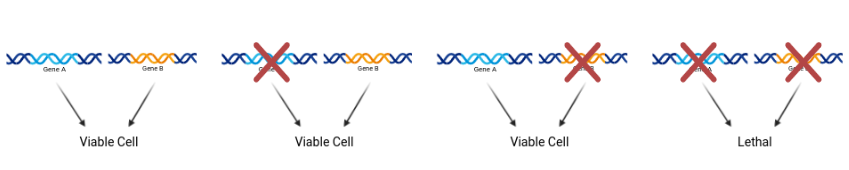
\includegraphics[width=11cm, height=2.5cm]{slbasic.png} 
		
			\item Inactivation: Preventing or disabling normal function of a gene (e.g mutation)
			\end{itemize}
			\centering
			\large \textbf{Synthetic = Combining}
			\footnotetext[2]{\tiny\cite{lee2018harnessing}}
	\end{frame}

	% SLIDE 4 - I do Not Know if I am including this slide
	% The Graphic for this slide is an  
	% Entropy, which is measured by Shannon's Entropy equation is a measure of compositional complexity which uses the proportion of residue(s)
	% in a subsequence to measure the compositional state of that subseequence - A lower variety of residues = lower entropy 
	%\begin{frame}{Shannon's Entropy - MAYBE }
		
	%		$H = -L\sum p_i log_2(p_i)$
		
	%\end{frame}

	%Slide 6
	% Poly(ADP-ribose) polymerases (PARPs) repair DNA SSBs through the BER pathway. PARP inhibitors, such as olaparib, prevent repair by trapping the inactivated PARP onto the SSB, resulting in the generation of DNA DSBs during the replication process. In tumors with a homologous recombination deficiency (HRD), such as a BRCA1/2 mutation, the low-fidelity repair mechanism of NHEJ leads to increasing genetic instability and ultimately death of the tumor cell.
	\begin{frame}{Recall: Synthetic Lethal Interactions are Harnessed for Precision Oncology}
		\begin{itemize} %(Olaparib, Niraparib, Rucaparib, Talazoparib)
			\item \small Four FDA approved anti-cancer drugs  are Poly [ADP-ribose] polymerase 1/2 (PARP1/2) inhibitors that work via a synthetic lethal mechanism
			
			\centering
			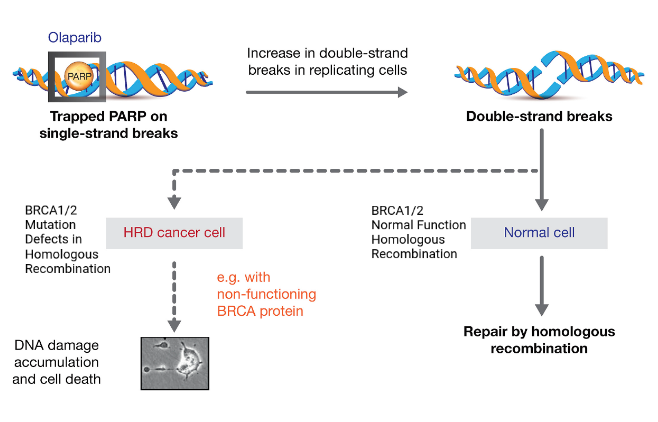
\includegraphics[width=8.5cm, height=6cm]{olaparib2.png}
			
			\footnotetext[4]{\tiny Figure From  \cite{o2015targeting}}
		\end{itemize}
		
	\end{frame}

	%EXPLAIN THE PROCESS OF ISLE HERE
	\begin{frame}{Recall: Building Pan-Cancer Synthetic Lethality Networks}
		\centering
		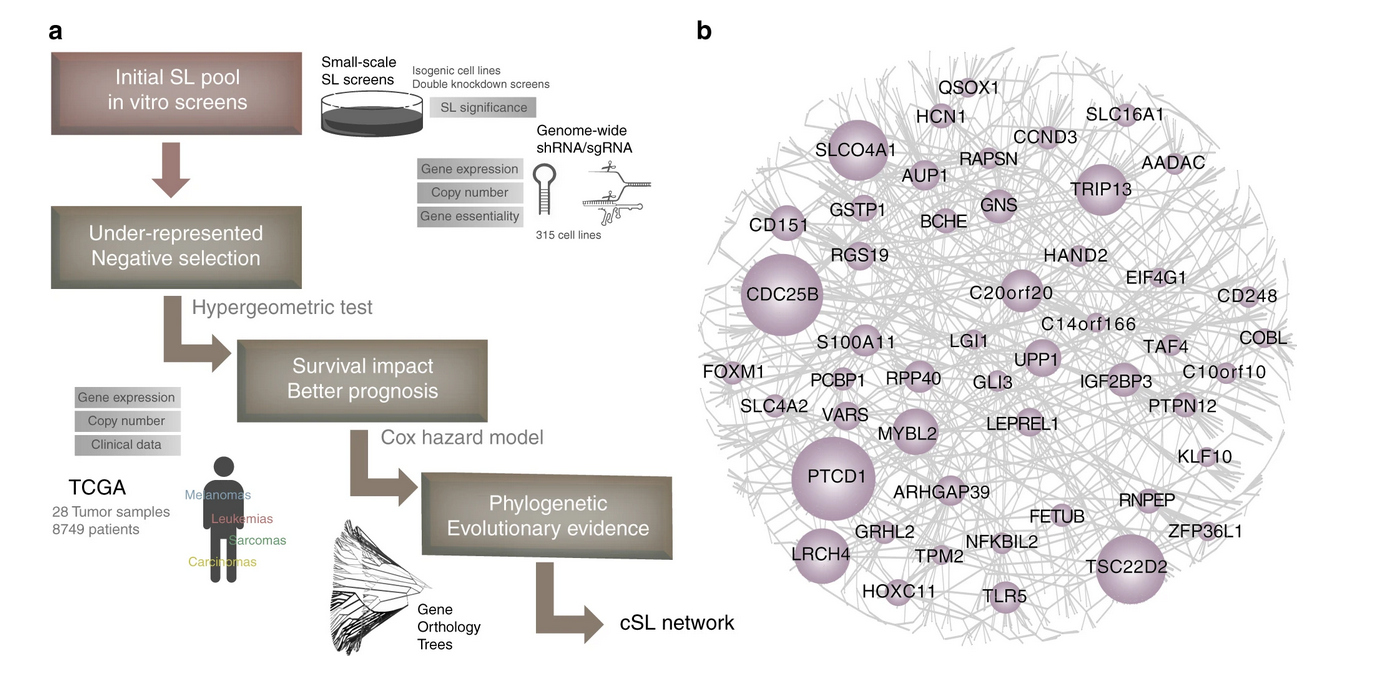
\includegraphics[width=13cm, height=7cm]{isle.png}
		%\movie[width=10cm,height=7cm,showcontrols=true]{\includegraphics[width=10cm, height=7cm]{pompe_thumbnail.png}}{pompe_trimmed.mp4}
		\footnotetext[2]{\tiny\cite{lee2018harnessing}}
	\end{frame}

	\begin{frame}{Recall: Sex Differences Add an Additional Layer of Complexity}
		Human sex differences are mainly caused by;
		\begin{enumerate}
			\item Gonadal hormone secretions
			\item Genes located on the sex chromosomes (X and Y) \newline
		\end{enumerate}
		This leads to differences in the frequency of certain cancer types and the efficacy of treatments in males and females
	\end{frame}

	\section{Approach}
	\begin{frame}{The Objective}
		\begin{center}
			%\includegraphics[width=11cm, height=6cm]{types_of_courses_taken.jpg}
			Can we build sex-specific synthetic lethality networks for various cancer types? \newline
			
			More specifically, we are trying to elucidate the differences in synthetic lethal interactions between males and females using a network based approach.
		\end{center}
	\end{frame}

	%%%%% APPRACH SECTION BEGINS HERE, 2 SLIDES
	
	\begin{frame}{Overall Project Workflow}
		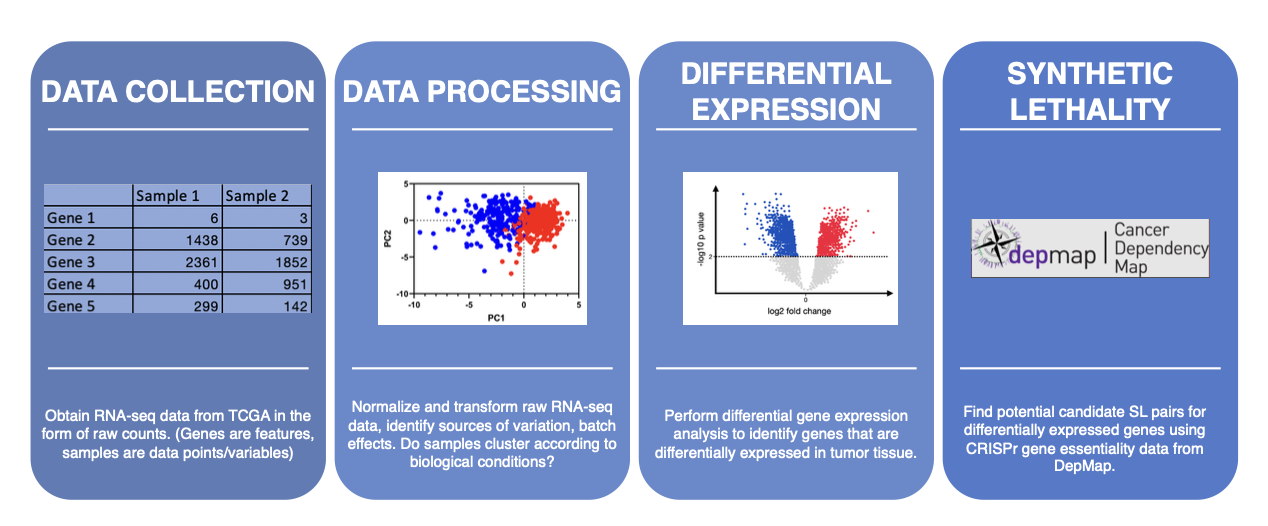
\includegraphics[width=12cm, height=5.2cm]{img2.png}
	\end{frame}

	\section{Data Collection}
	\begin{frame}{Selection of TCGA Cancer Types}
			\begin{columns}
				\begin{column}{0.45\textwidth}
					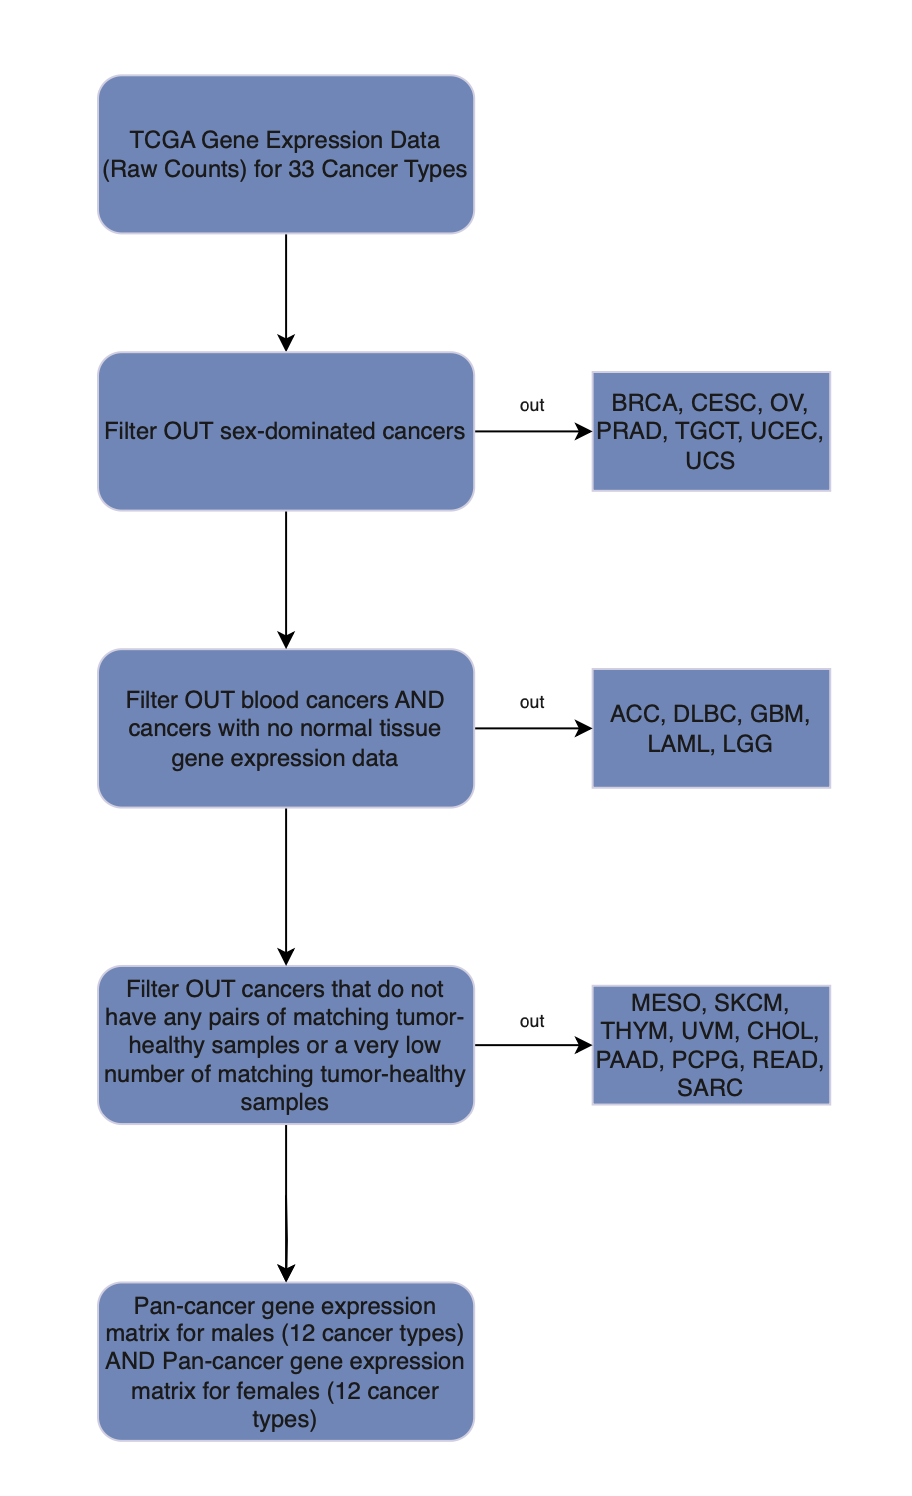
\includegraphics[width=5cm, height=8cm]{img3.png}
				\end{column}
				\begin{column}{0.5\textwidth}
					\begin{itemize}
						\item There is a lack of healthy tissue RNA-seq samples in the TCGA database (12 cancers with more than 10 pairs in M and F)
						\item Raw count pan-cancer matrices created with 12 remaining TCGA cancer types (BLCA, COAD, ESCA, HNSC, KICH, KIRC, KIRP, LIHC, LUAD, LUSC, STAD, THCA)
					\end{itemize}
				\end{column}
			\end{columns}			
	\end{frame}

	\begin{frame}{Creating and Pre-Filtering Pan-Cancer Expression Matrices}
		\begin{itemize}
			\item For each gene, if expression is $>$ 90th quantile of overall expression in AT LEAST 1 sample, we keep it, otherwise we filter it out
			\item We reduce the amount of genes with extremely low expression, thereby reducing noise and improving sensitivity to detect differentially expressed genes (genes with weak expression are more susceptible to technical noise arising from library size, library composition, etc)
		\end{itemize}
	\end{frame}

	%Both samples are sequenced at the same depth - sample A has 5 genes expressed at same level, Sample B has the same genes as sample A plus two highly expressed genes that take up 50% of the reads
	\section{Data Processing}
	\begin{frame}{Normalization for RNA-seq Data Analysis}
		\centering Required to identify genes that are differentially expressed due to some biological phenomena and not due to technical variation
		
		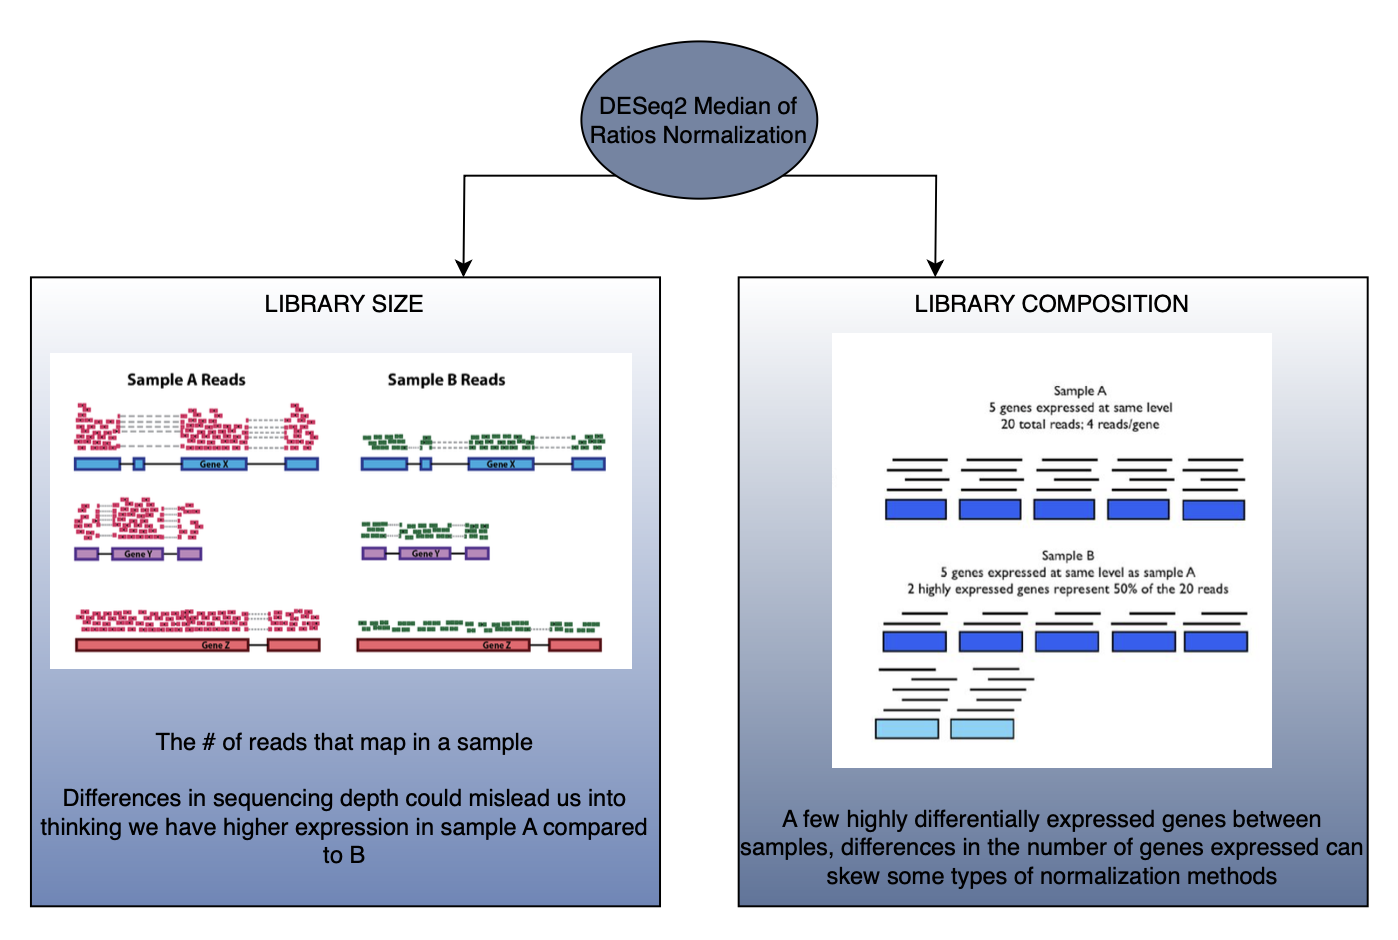
\includegraphics[width=9cm,height=7cm]{img4.png}
	\end{frame}

	\begin{frame}{Normalizing Pan-Cancer Expression Matrices}
		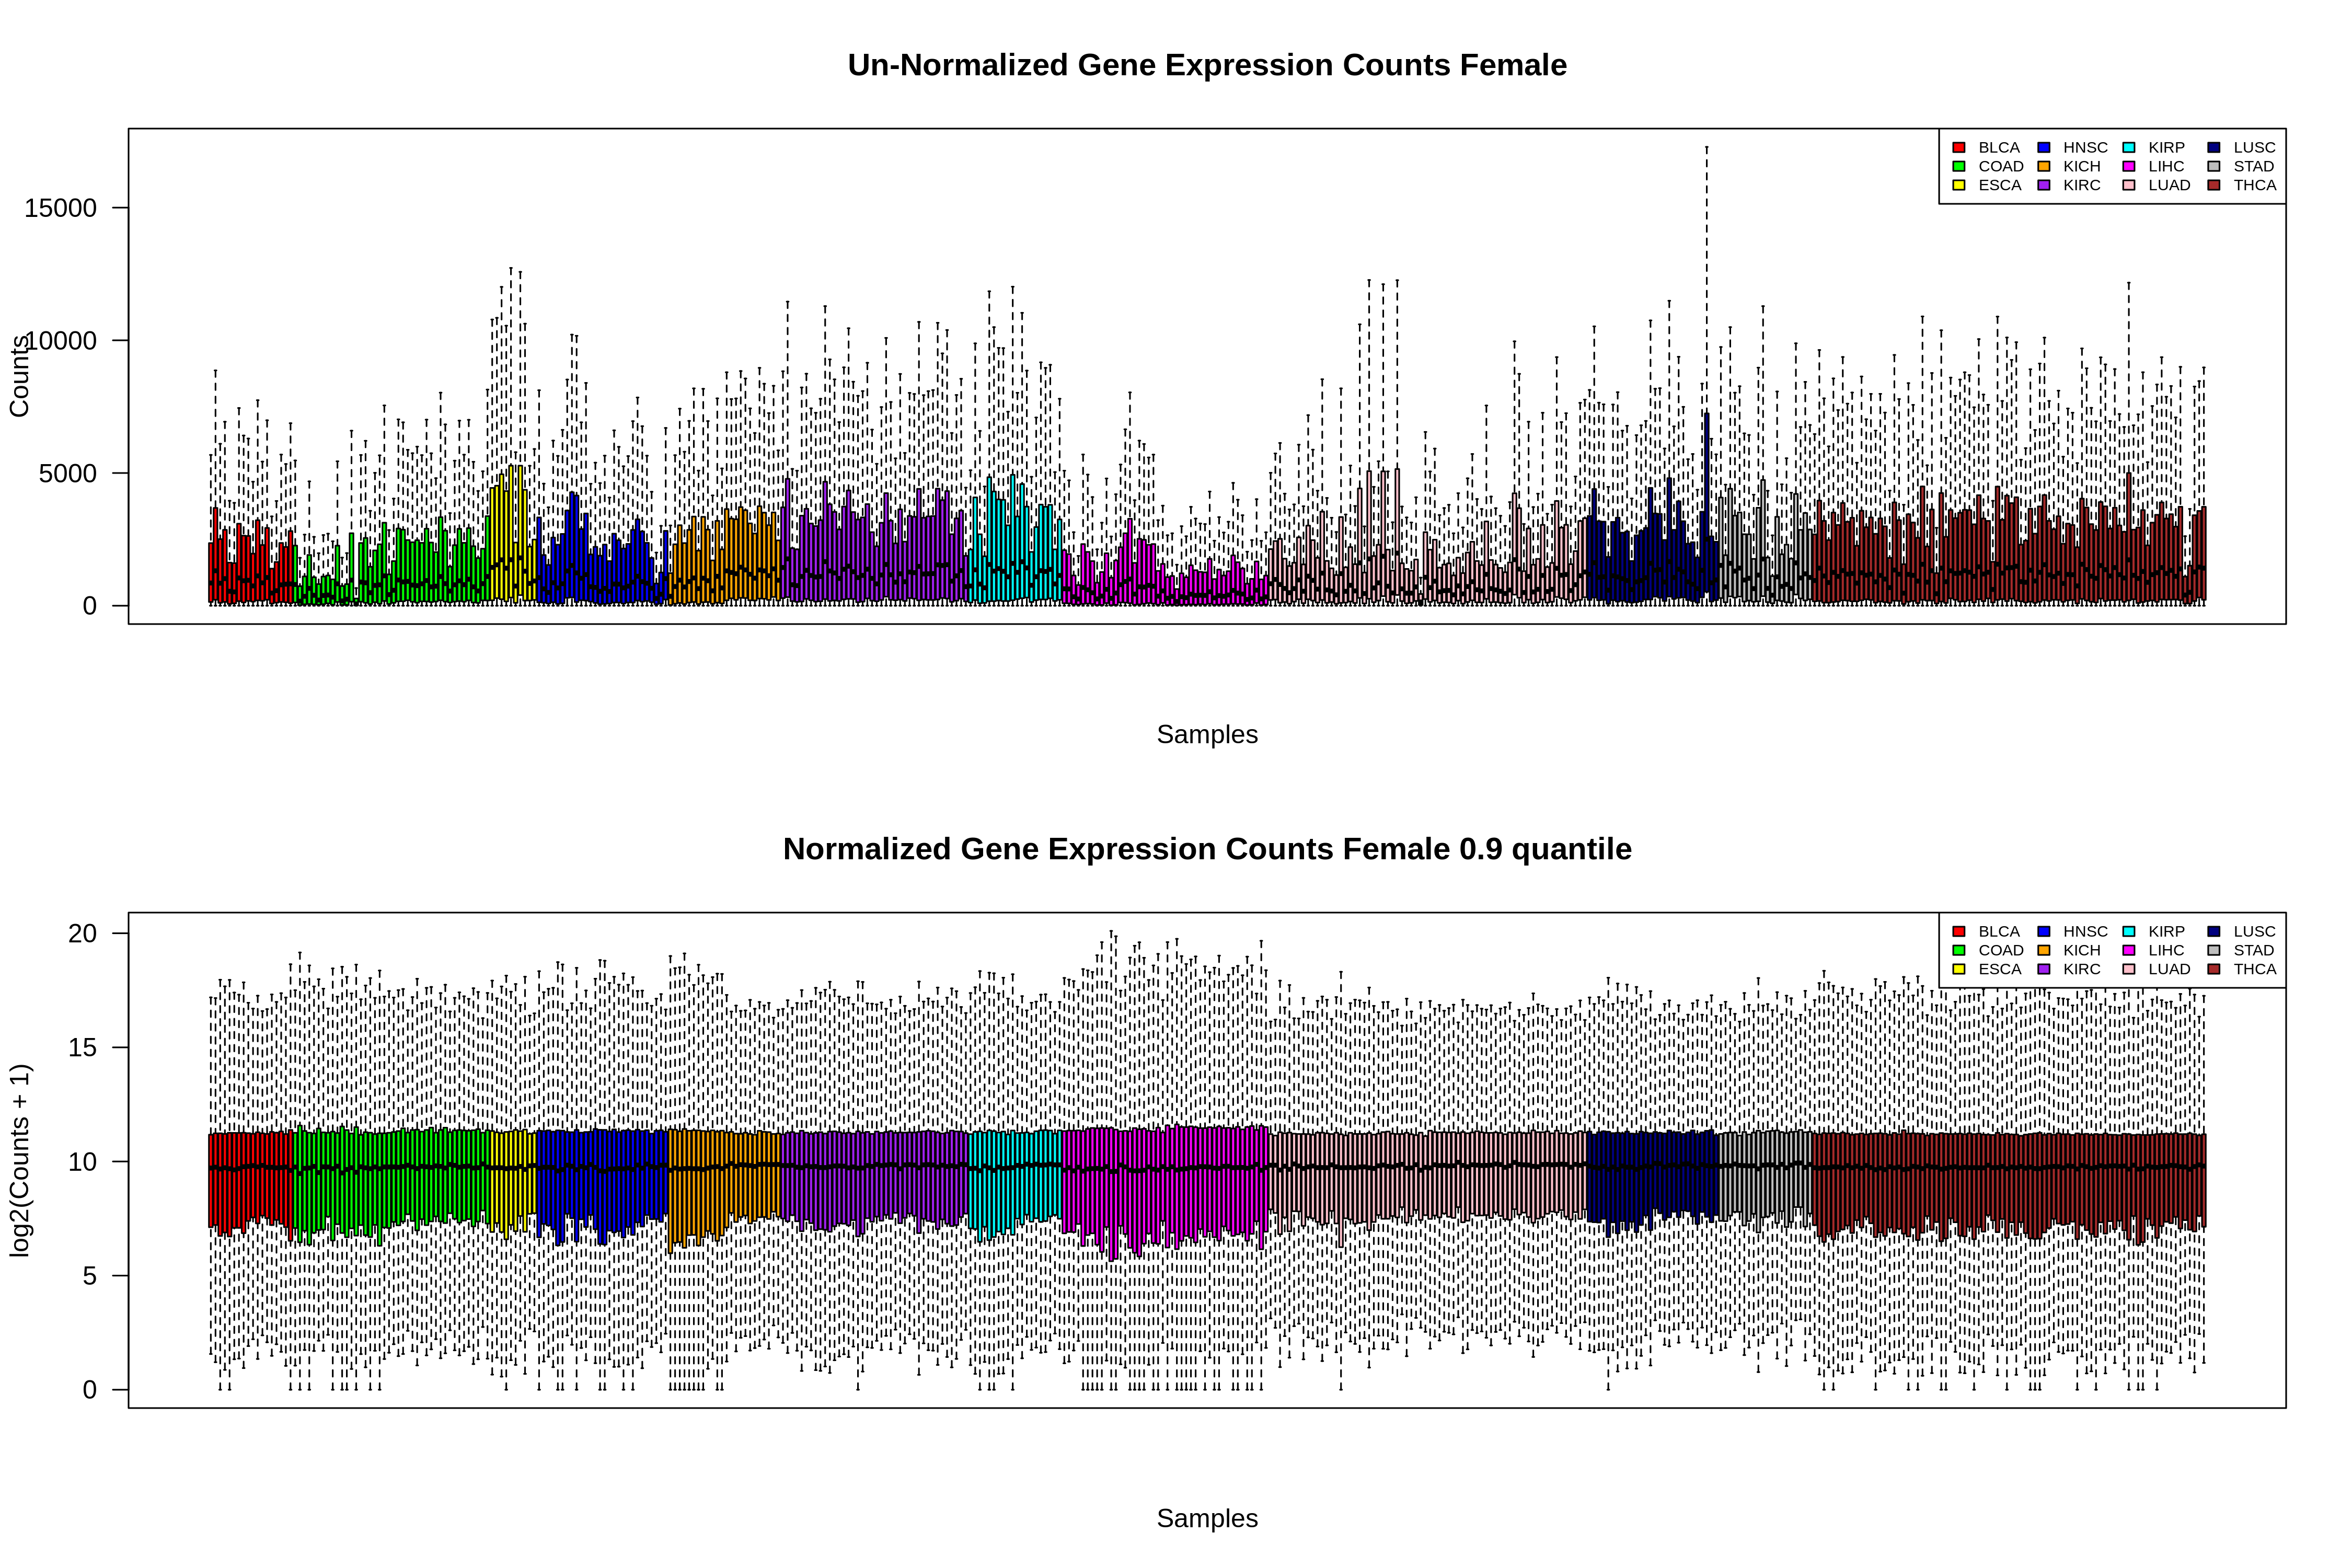
\includegraphics[width=12cm, height=8cm]{all_cancers-F_before_and_after_normalization_v.png}
	\end{frame}

	\section{Data Processing}
	\begin{frame}{Normal and Tumor Tissue Differ ACROSS 12 Cancer Types}
		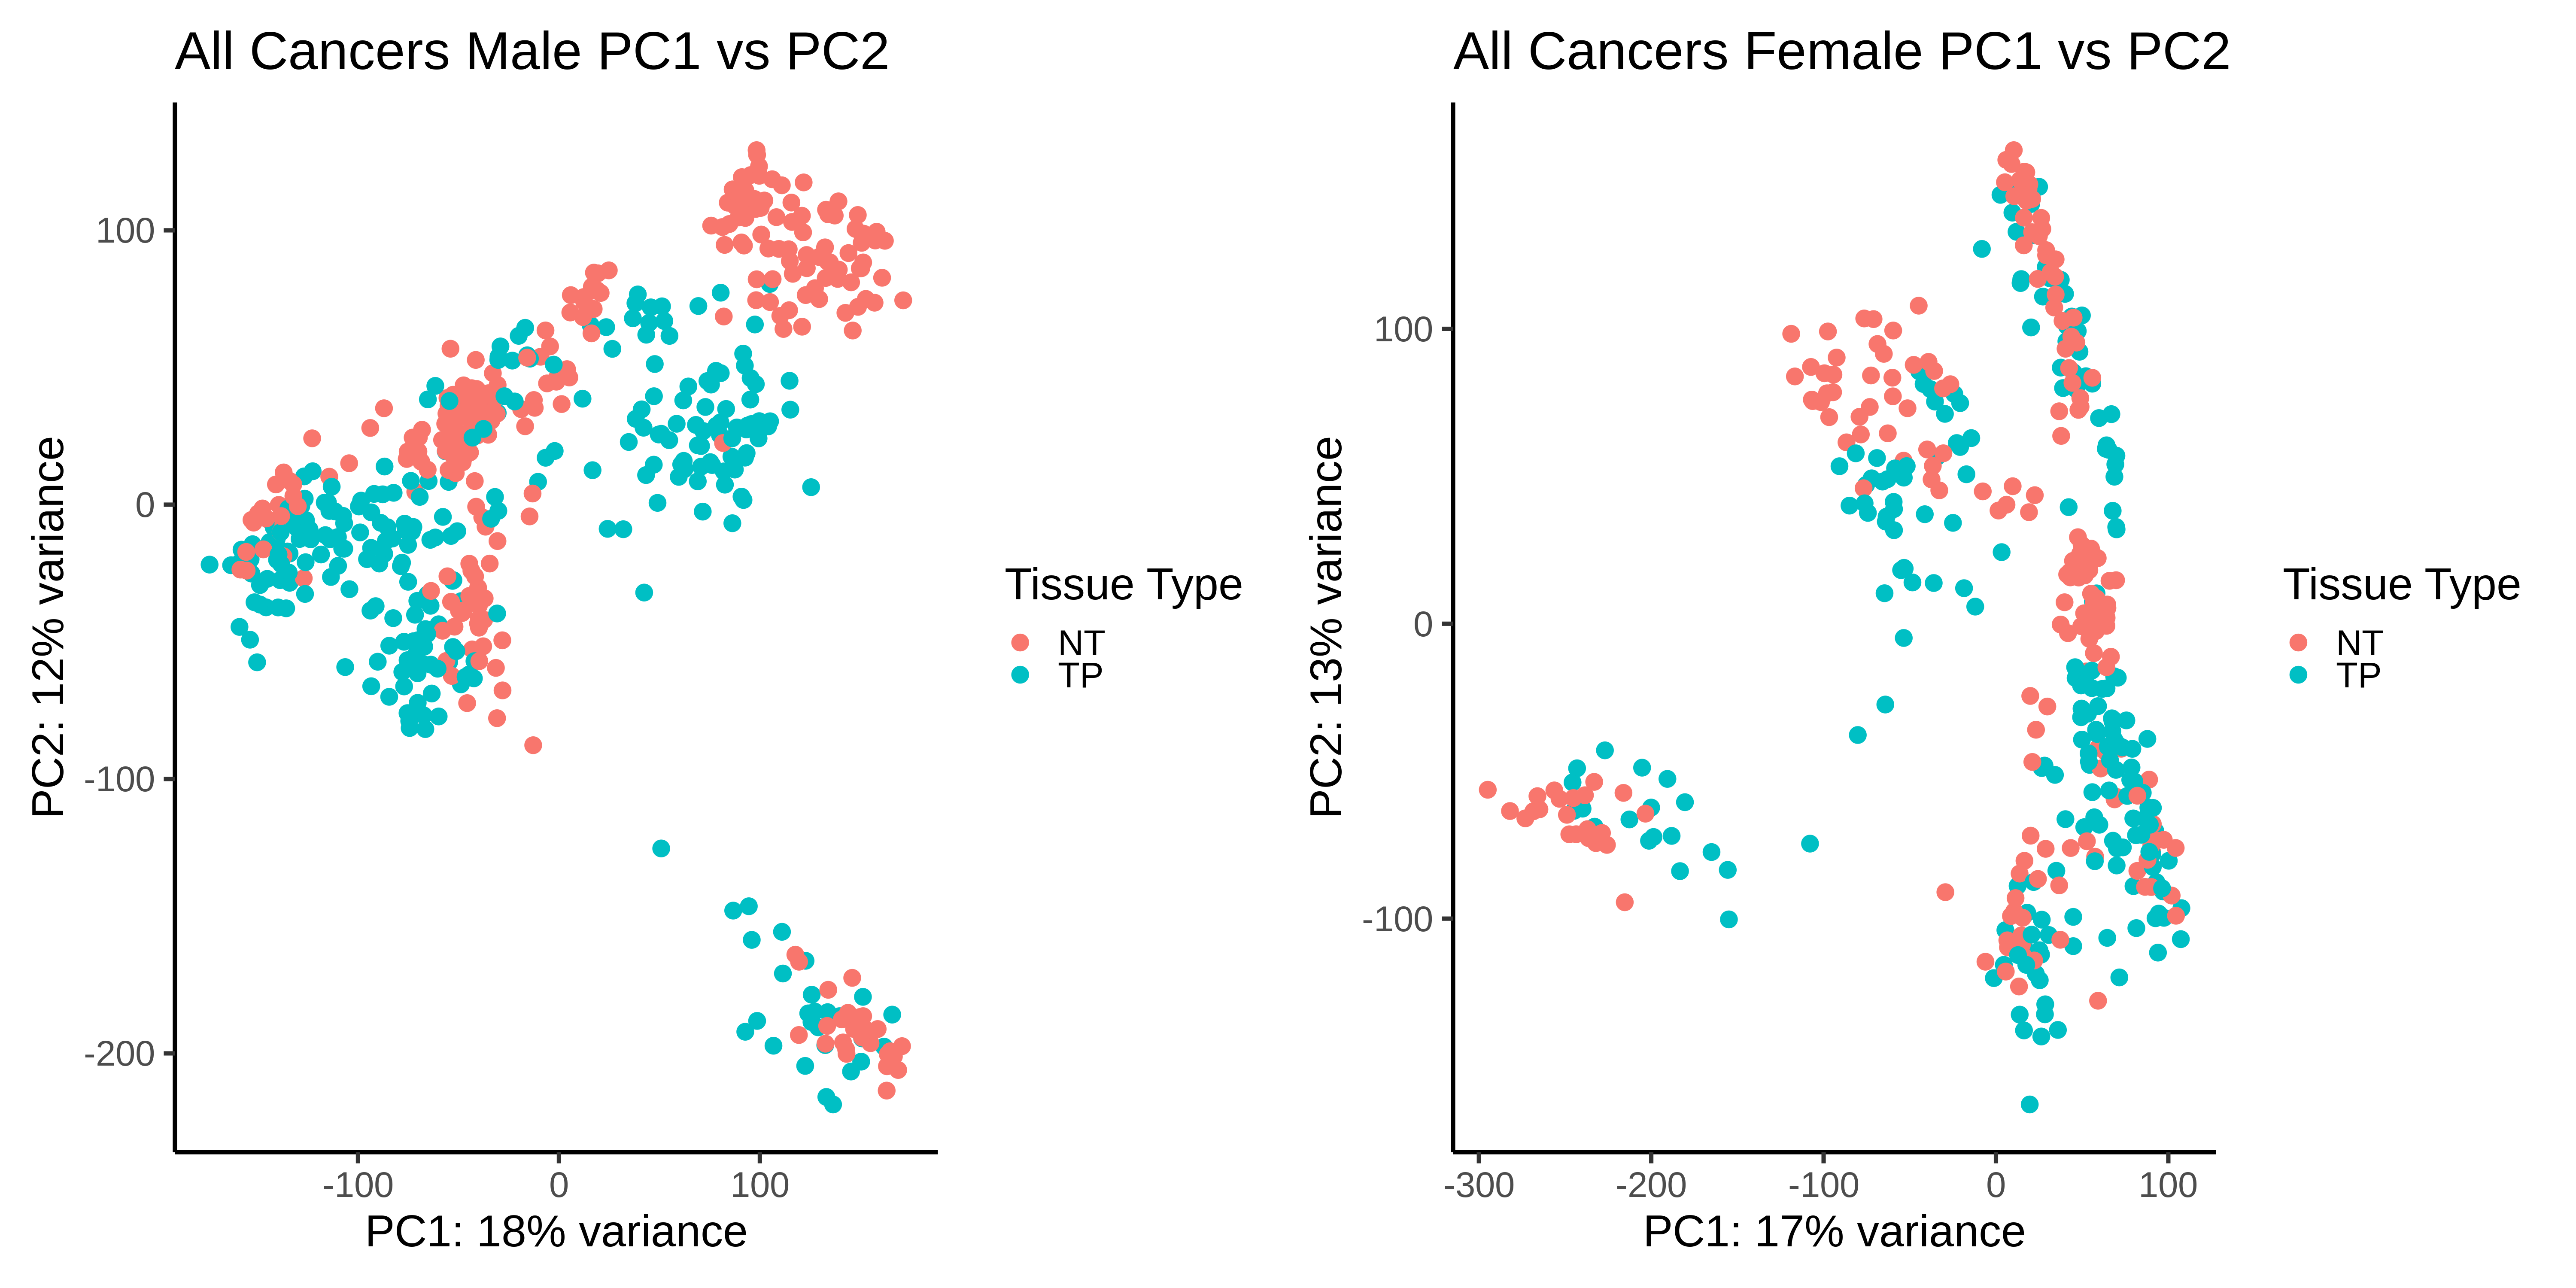
\includegraphics[width=12cm, height=6cm]{all_cancerspca_analysis_condition_0.9.png}
		
		Across all 12 cancer types, the observed variation between healthy and tumor tissue samples is unlikely to have occurred by chance alone (NPManova p-val = 0.0001)
	\end{frame}

	\begin{frame}{Normal and Tumor Tissue Differ WITHIN each Cancer}
		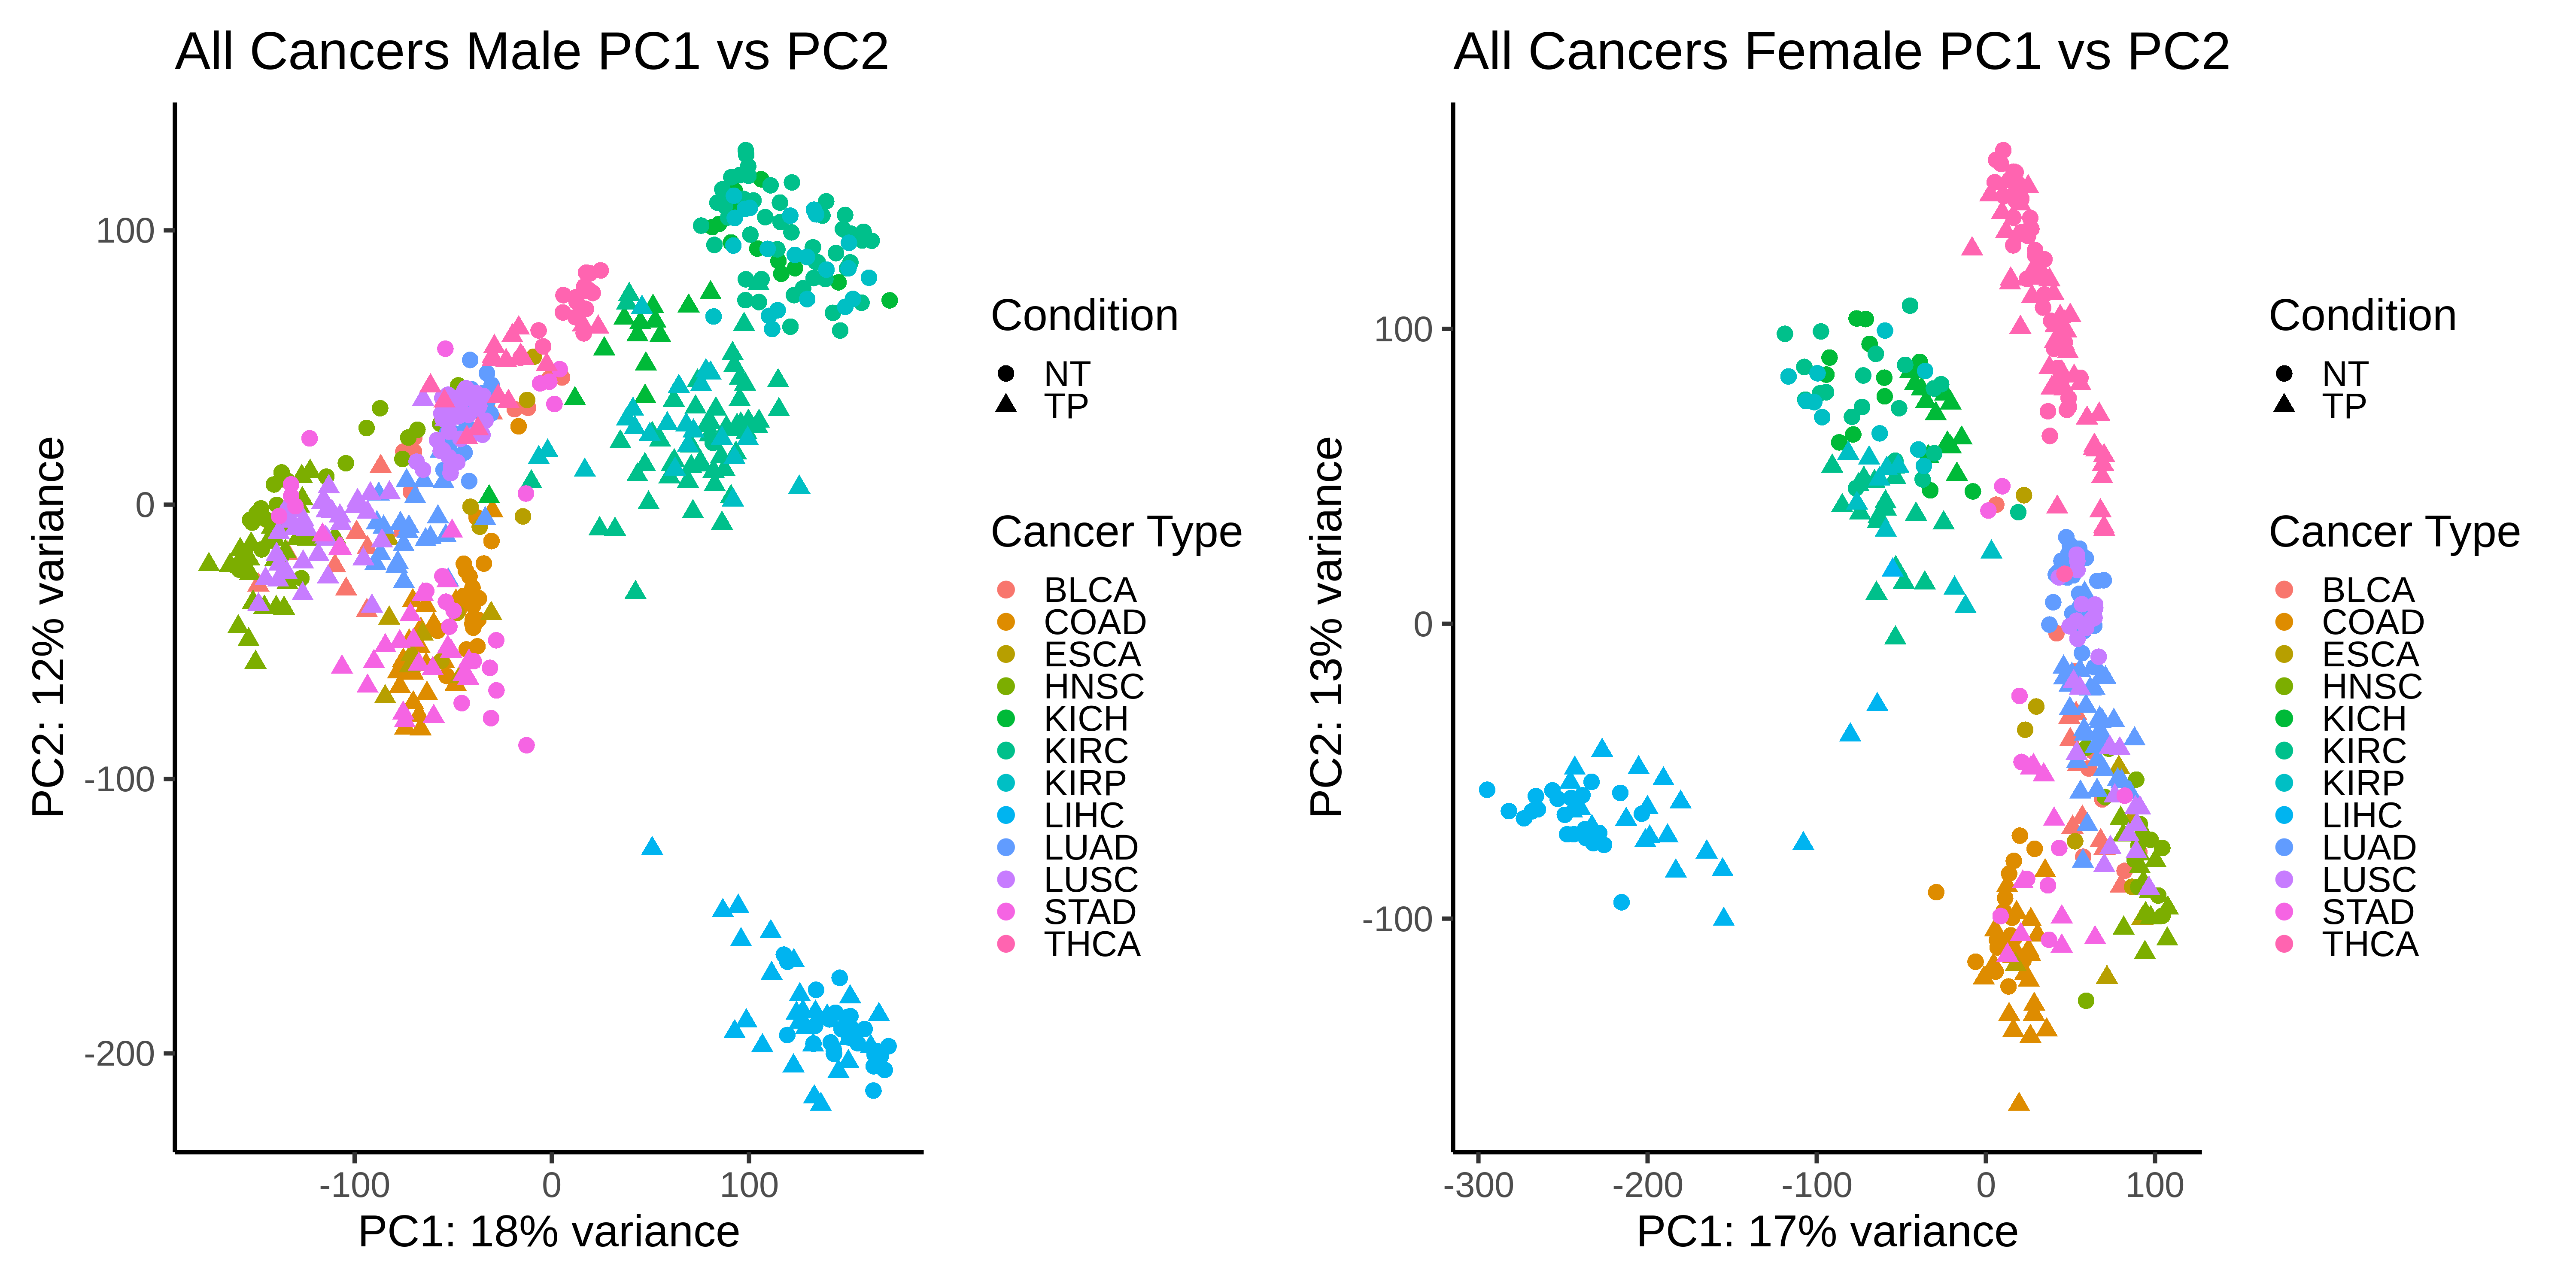
\includegraphics[width=12cm, height=6cm]{all_cancerspca_analysis_condition_cancertype_0.9.png}
		
		Within each cancer type, the observed variation between healthy and tumor tissue samples is unlikely to have occurred by chance alone (Acceptions: Males: ESCA (LOW SAMPLE SIZE), Females: BLCA, ESCA (LOW SAMPLE SIZE), STAD (LOW SAMPLE SIZE))
	\end{frame}


	\section{Differential Expression}
	%Our data do not fit the Poisson distribution
	%(i.e. Poisson will underestimate variability leading to an increase in false positive DE genes).
	\begin{frame}{Why does DESeq2 Use the Negative Binomial Distribution}
		\begin{itemize}
			\item Reads are count based hence they cannot be normally distributed
			\item Variance tends to be greater than the mean, especially for genes with large mean expression values
			\item  We need to account for this increase in variance using the Negative Binomial model 
		\end{itemize}
	\centering 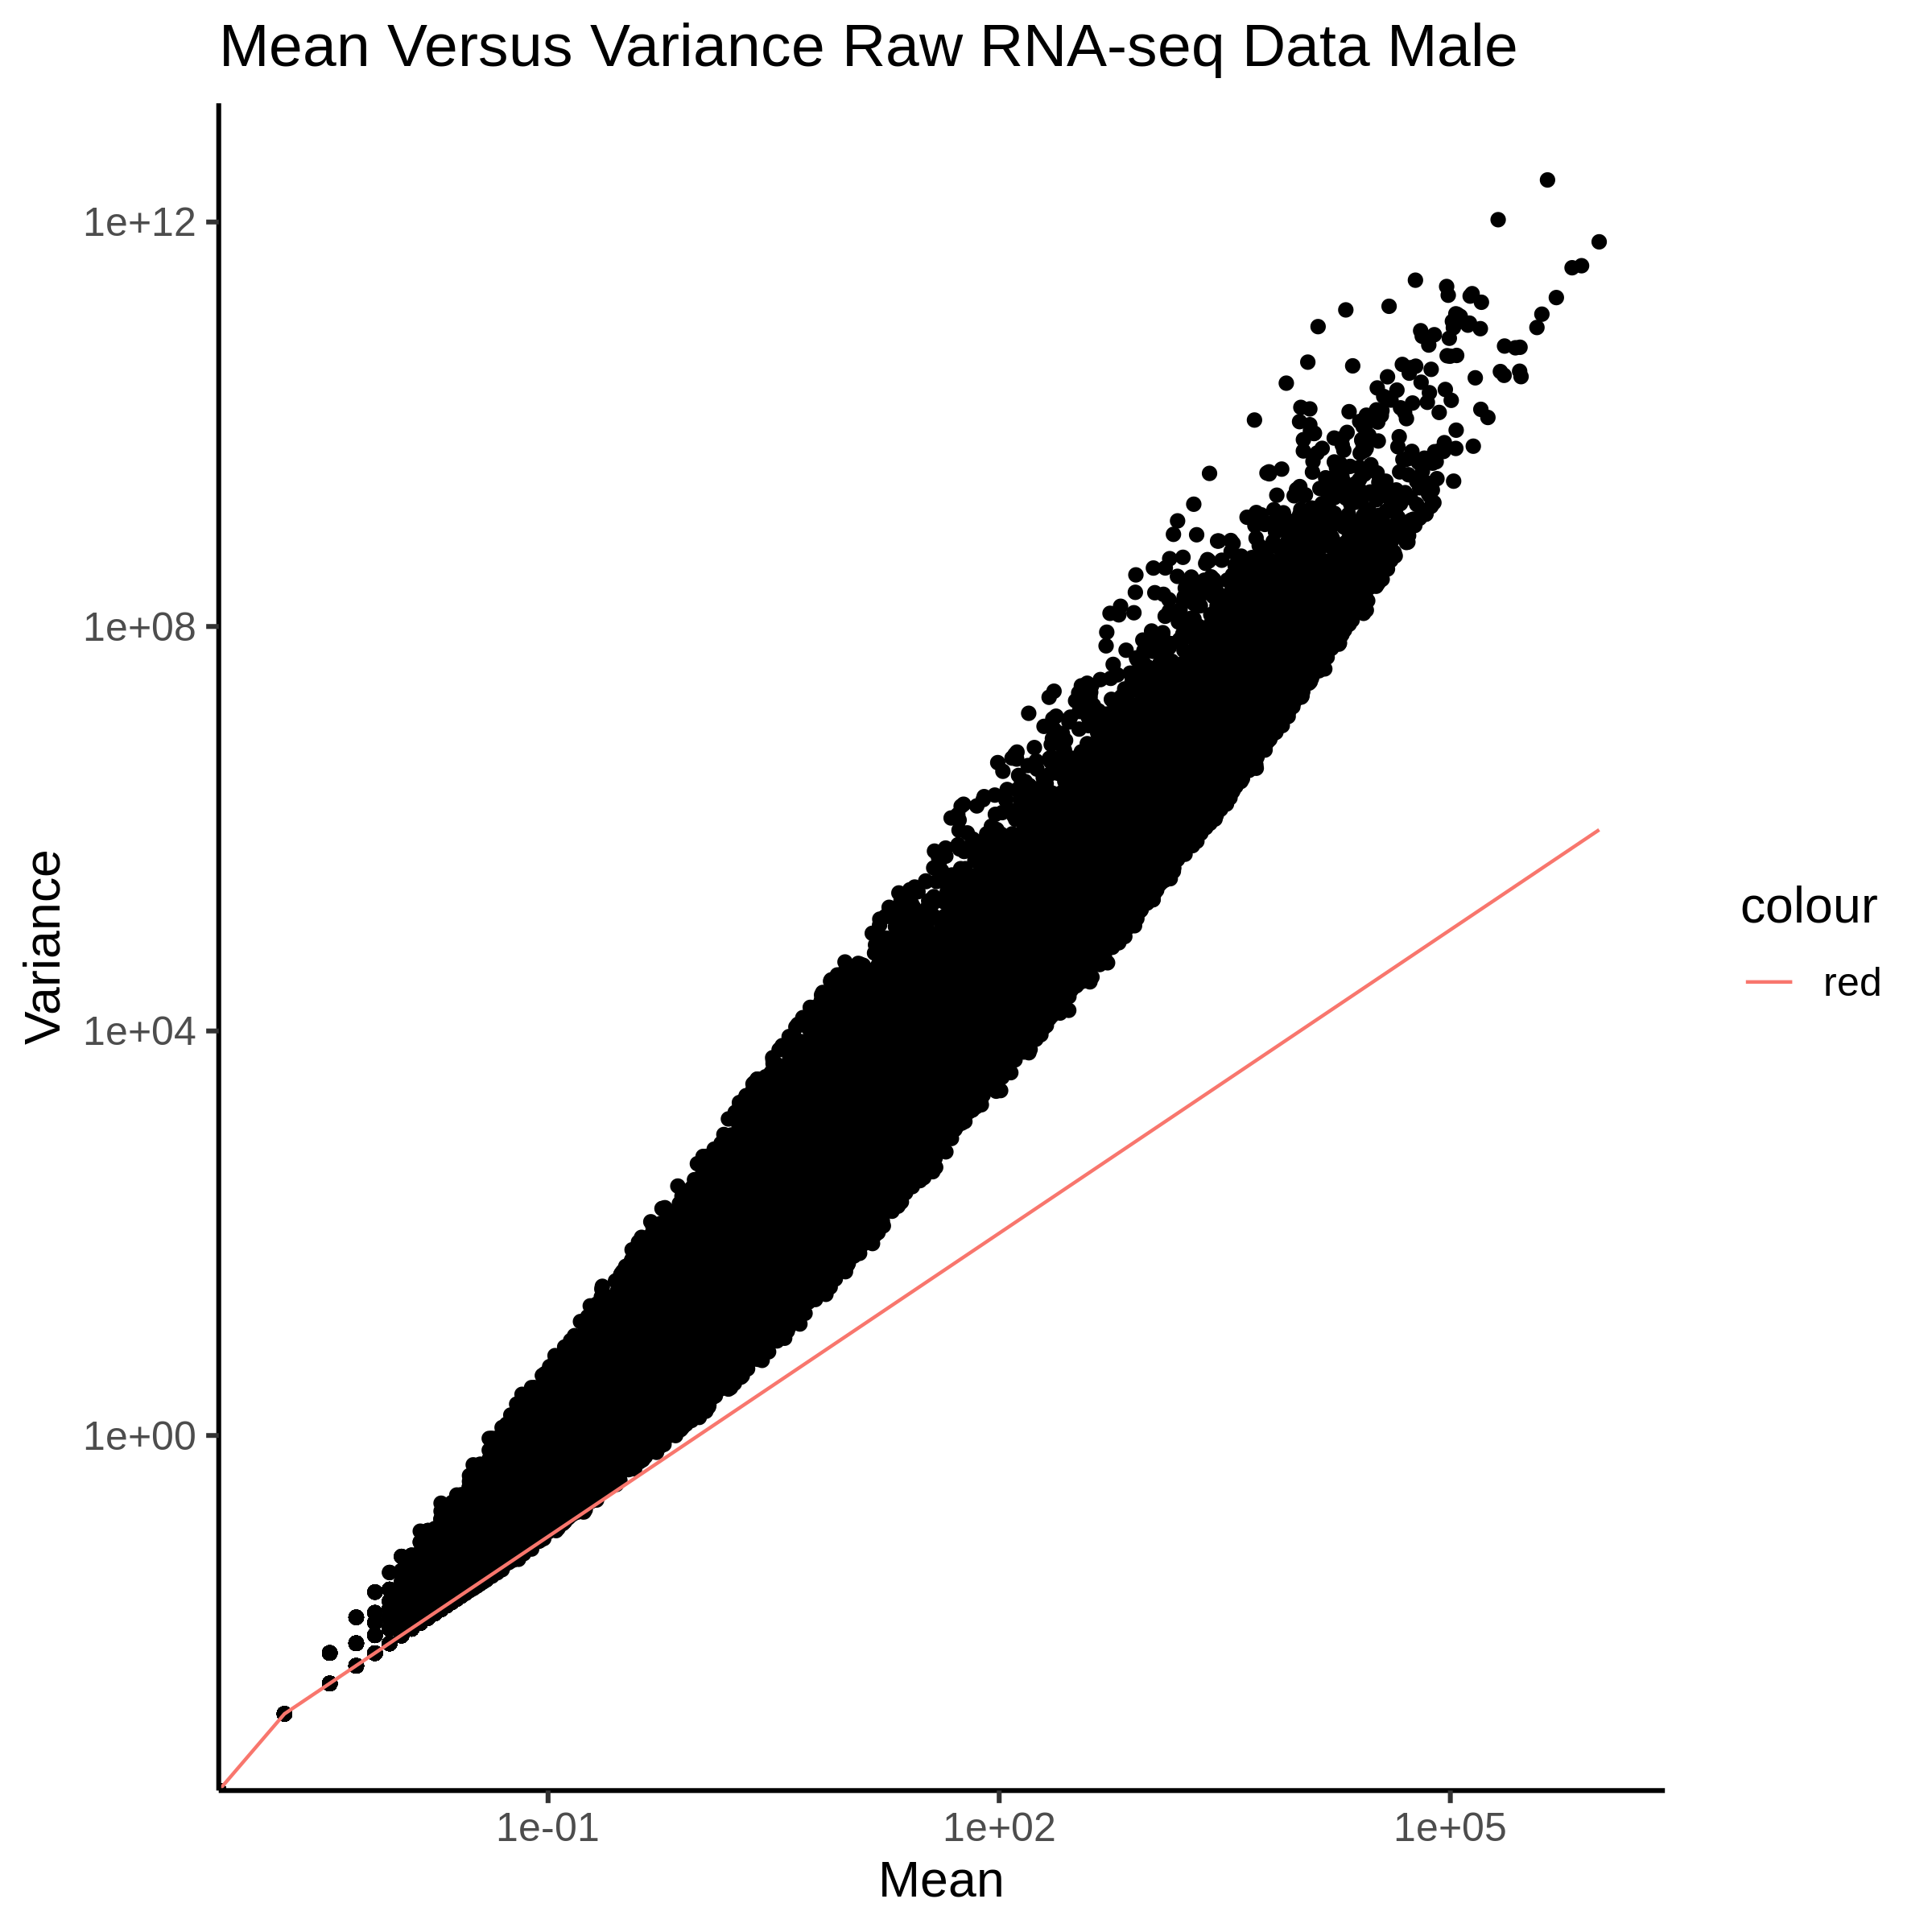
\includegraphics[width=5.5cm, height=5.5cm]{all_cancersmean_vs_variance_male.png}
	\end{frame}

	\begin{frame}{DESeq2 Accounts for Increased Variance}
		\begin{enumerate}
			\item Estimate gene-wise dispersions: captures biological variability in gene expression across samples
			\item Fit negative binomial GLM to count data: This model incorporates the estimated gene-wise dispersions as a parameter to account for variability in the data
			\item Use fitted GLM to identify differentially expressed genes \newline
		\end{enumerate}
		The use of linear models allows for more complex designs \newline \newline
		$design = ~cancertype + condition$ \newline \newline
		This tells DESeq2 to test the effect of condition while controlling for the effect of cancer type
	\end{frame}

	\begin{frame}{Finding Differentially Expressed Genes (DESeq2)}
		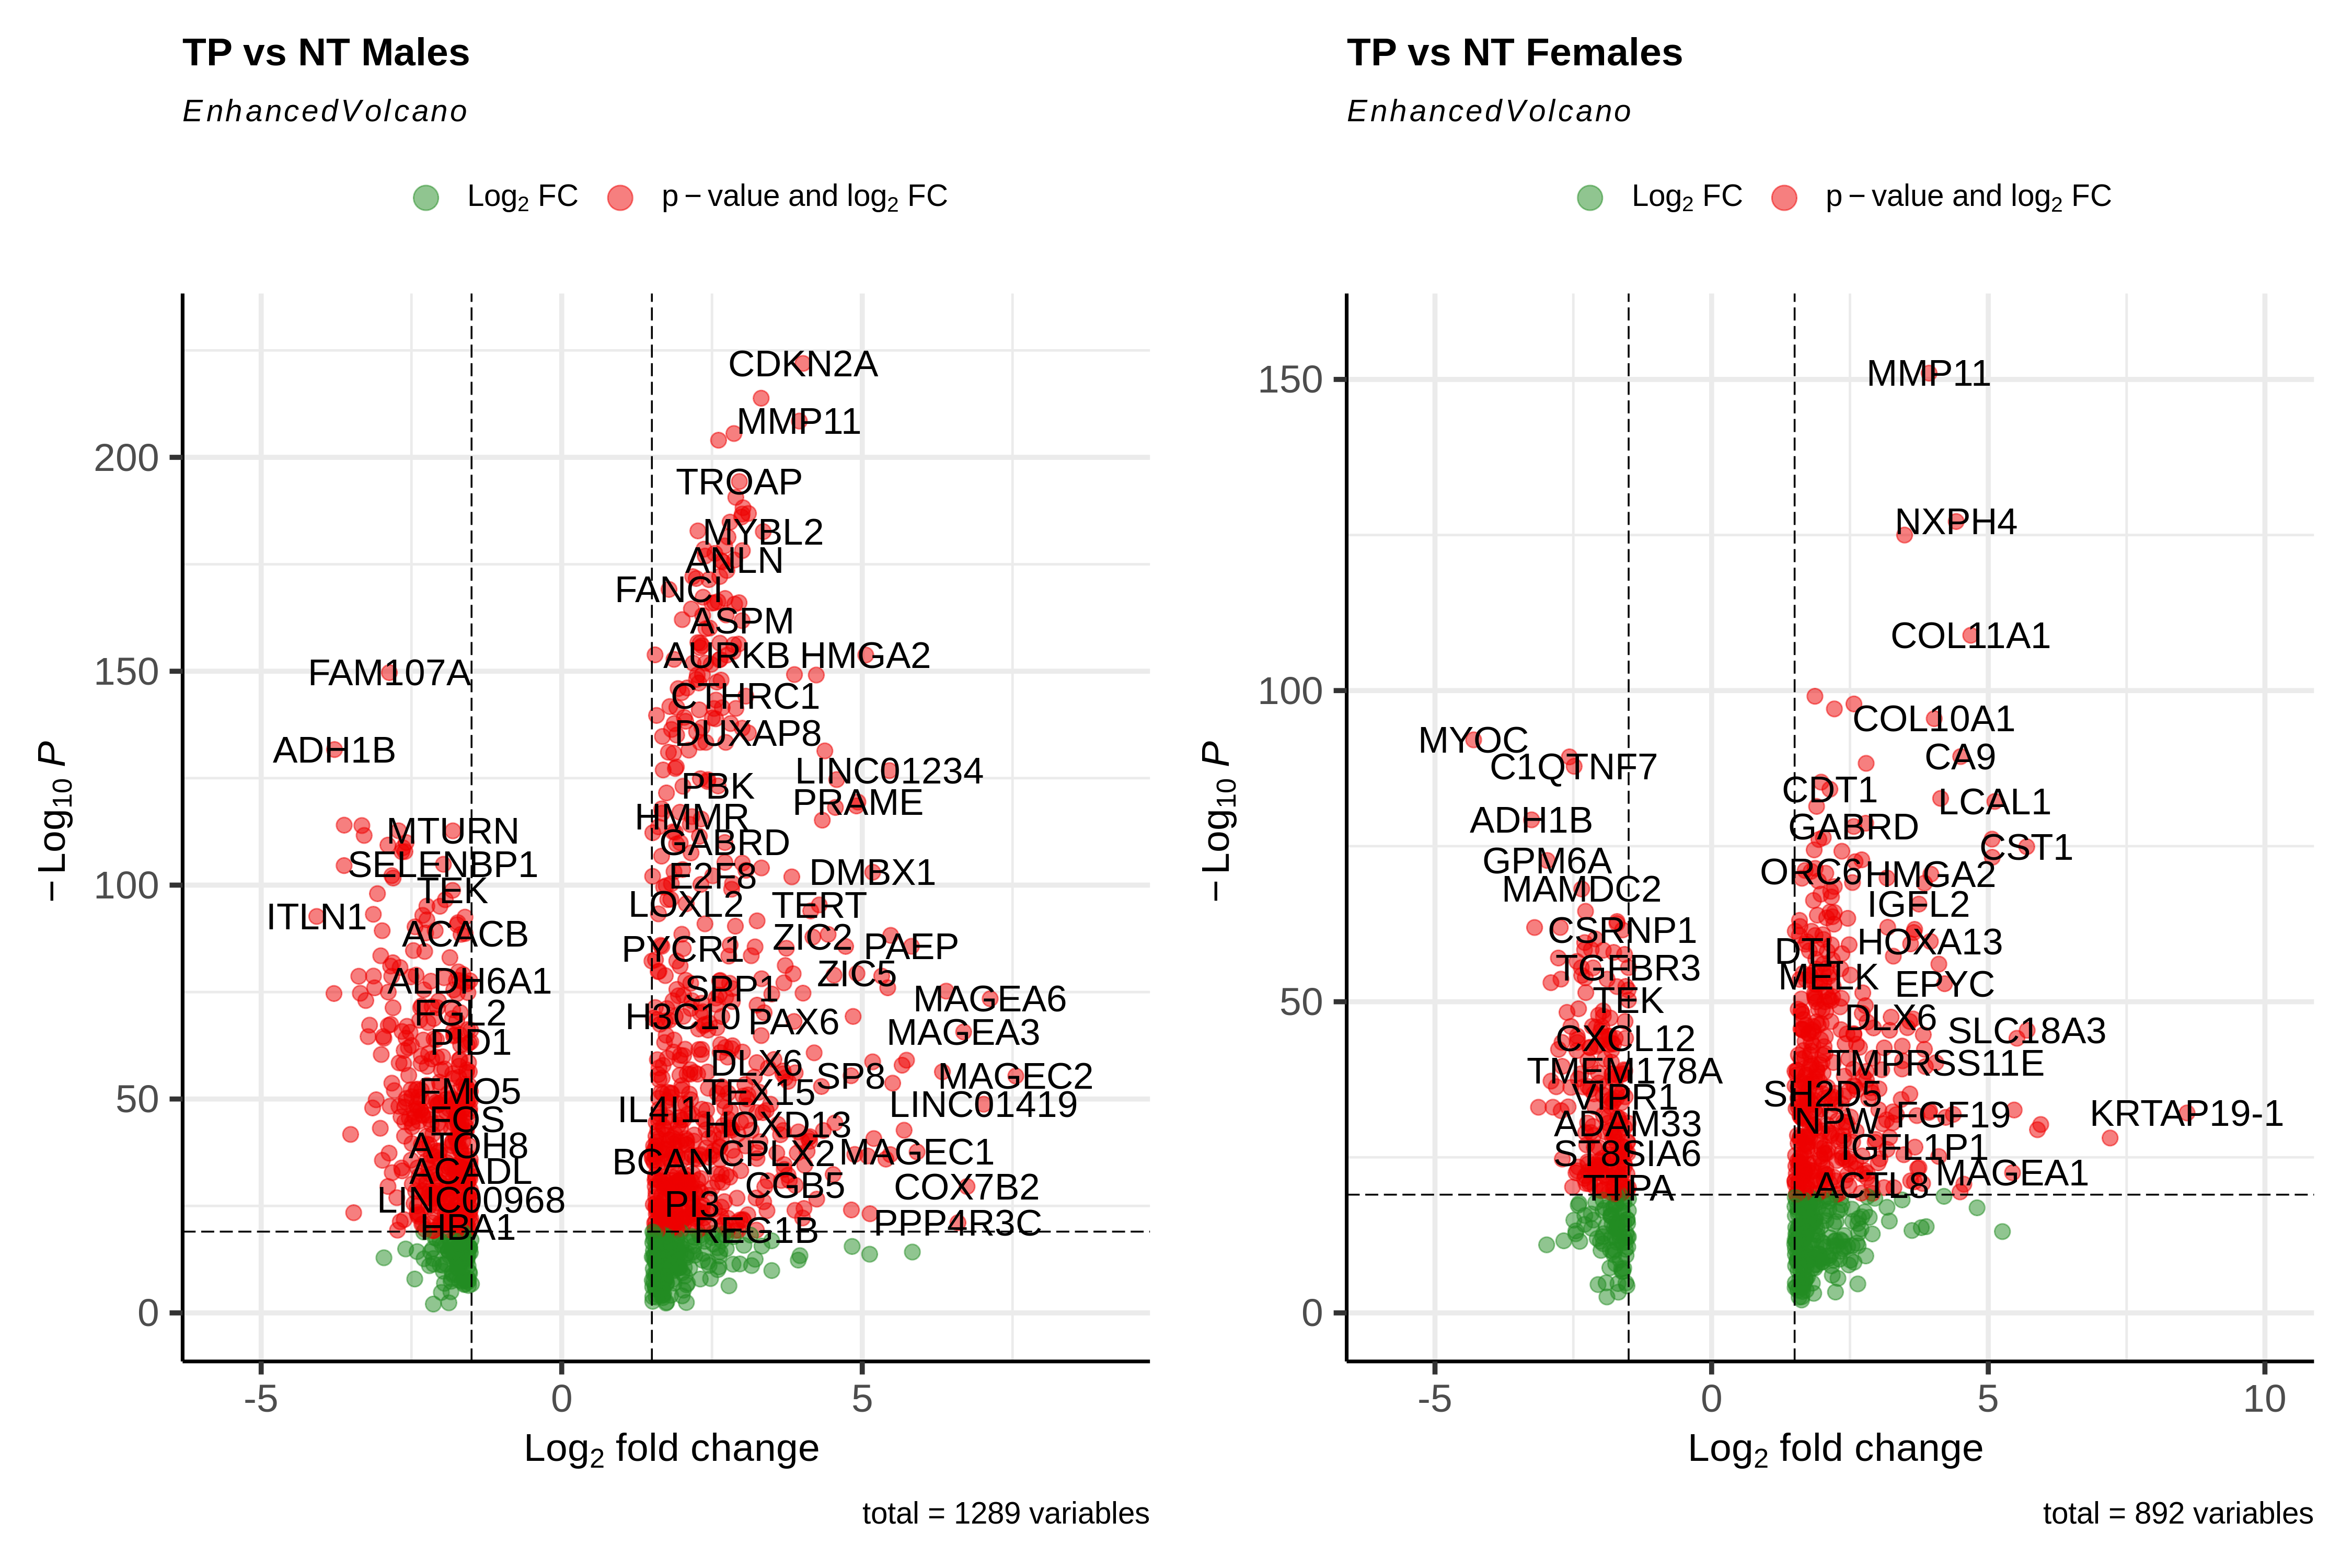
\includegraphics[width=12cm, height=8cm]{all_cancersvolcano_analysis_0.9.png
		}
	\end{frame}

	\begin{frame}{Differences in Number of DE Genes Males vs Females}
		\centering 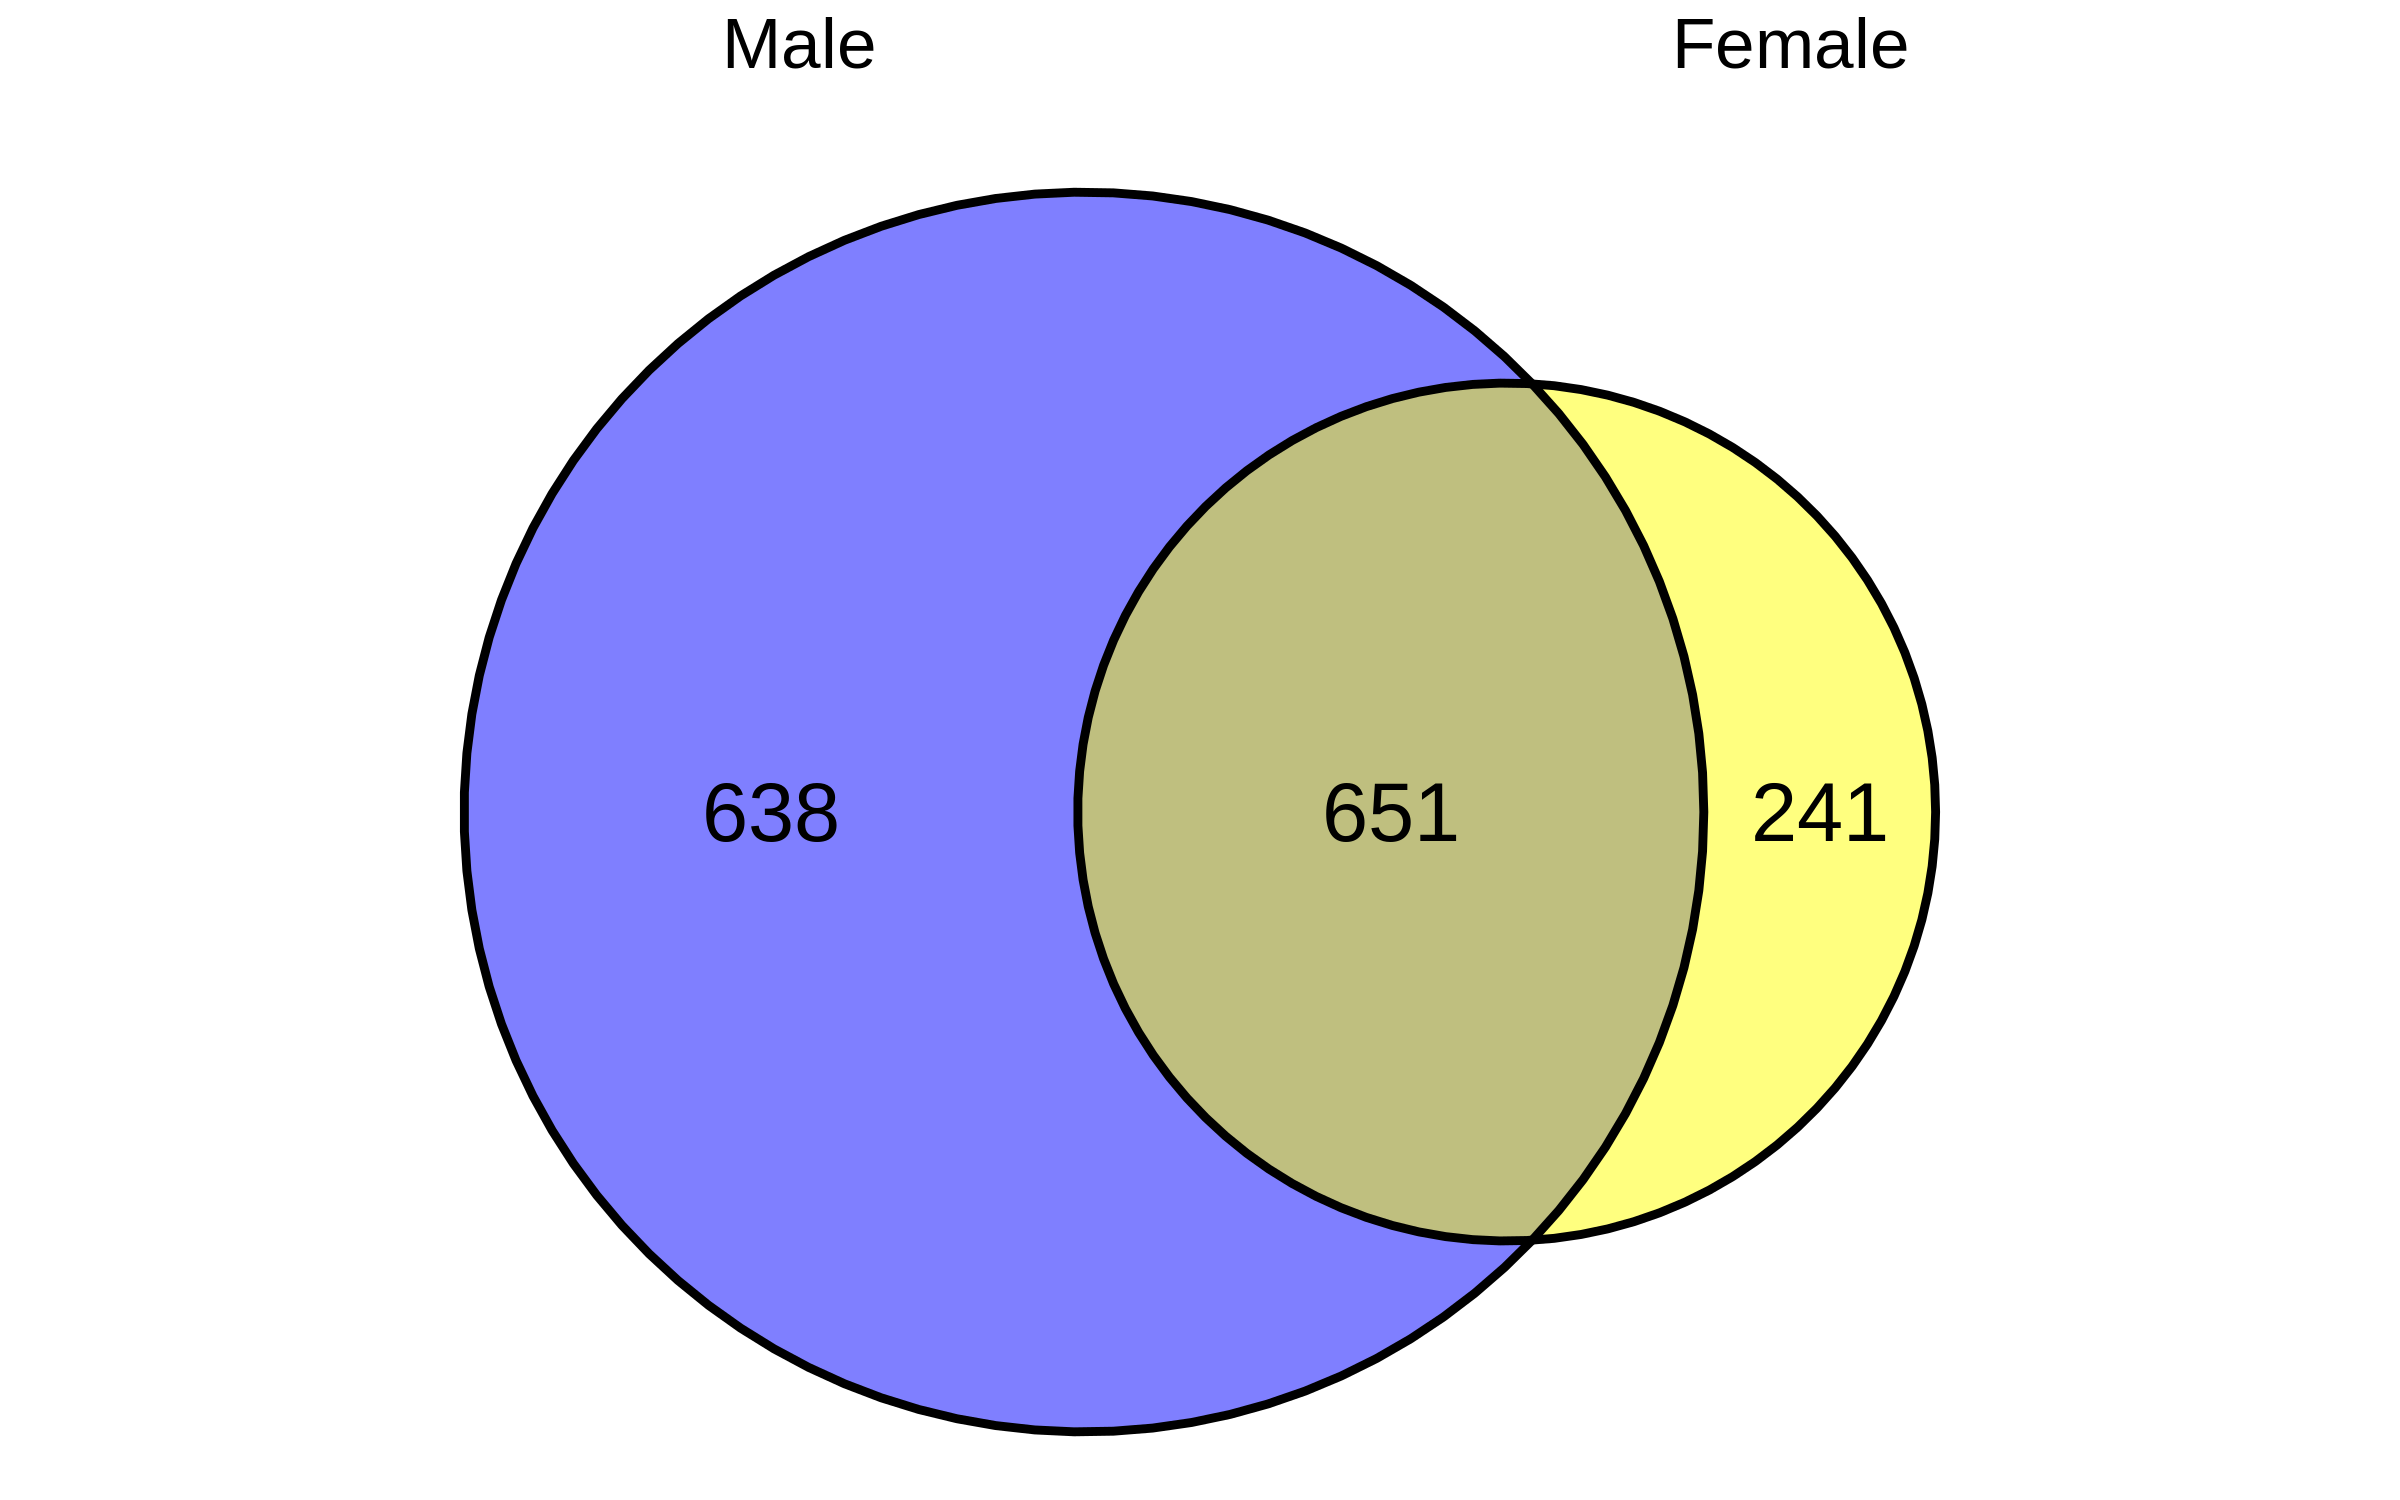
\includegraphics[width=9cm, height=5cm]{all_cancersvenndiagram_malede_vs_femalede_0.9.png}
		\begin{itemize}
			\item \textcolor{blue}{MALES: 358 up-regulated in tumor, 280 Down-regulated in tumor}
			\item \textcolor{yellow}{FEMALES: 171 up-regulated in tumor, 70 down-regulated in tumor}
		\end{itemize}
	\end{frame}

	\begin{frame}{DE Genes Found in Males and Females are Enriched in Cancer-Related Processes}
		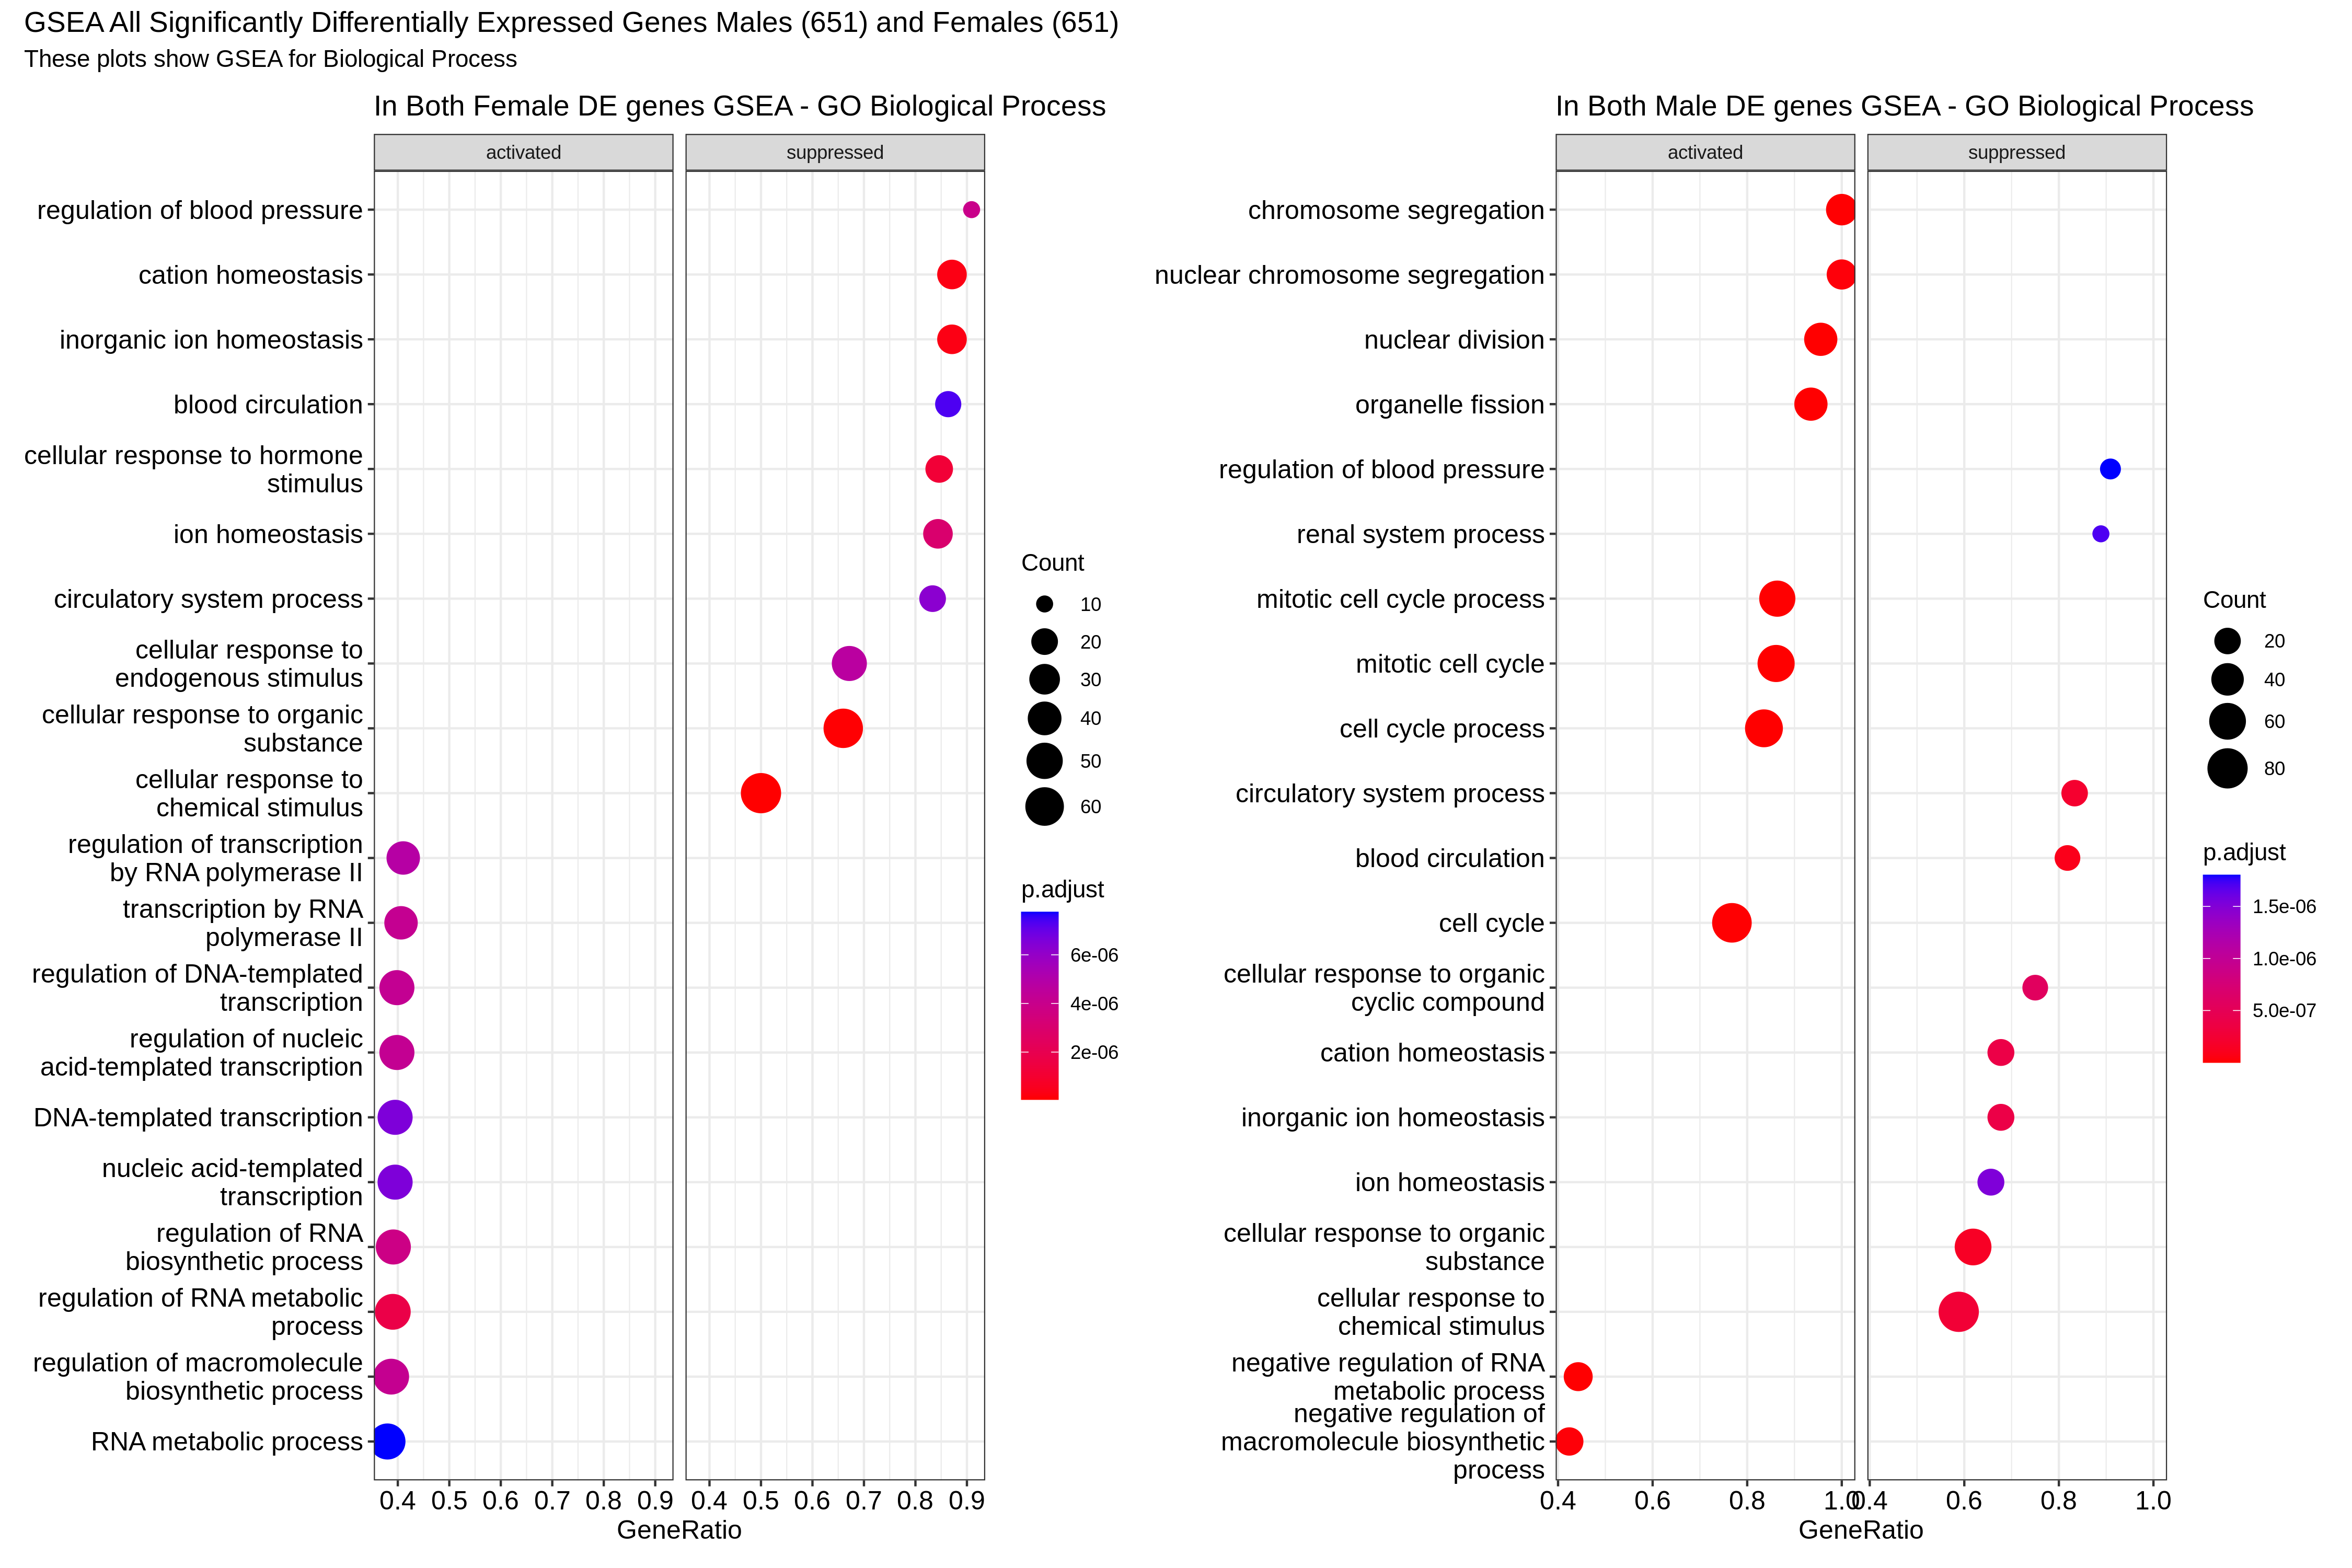
\includegraphics[width=11cm, height=7cm]{all_cancersgsea_inbothdegenes_male_female_bp0.9.png}
	\end{frame}

	\begin{frame}{Enriched Biological Processes Differ in Males and Females}
		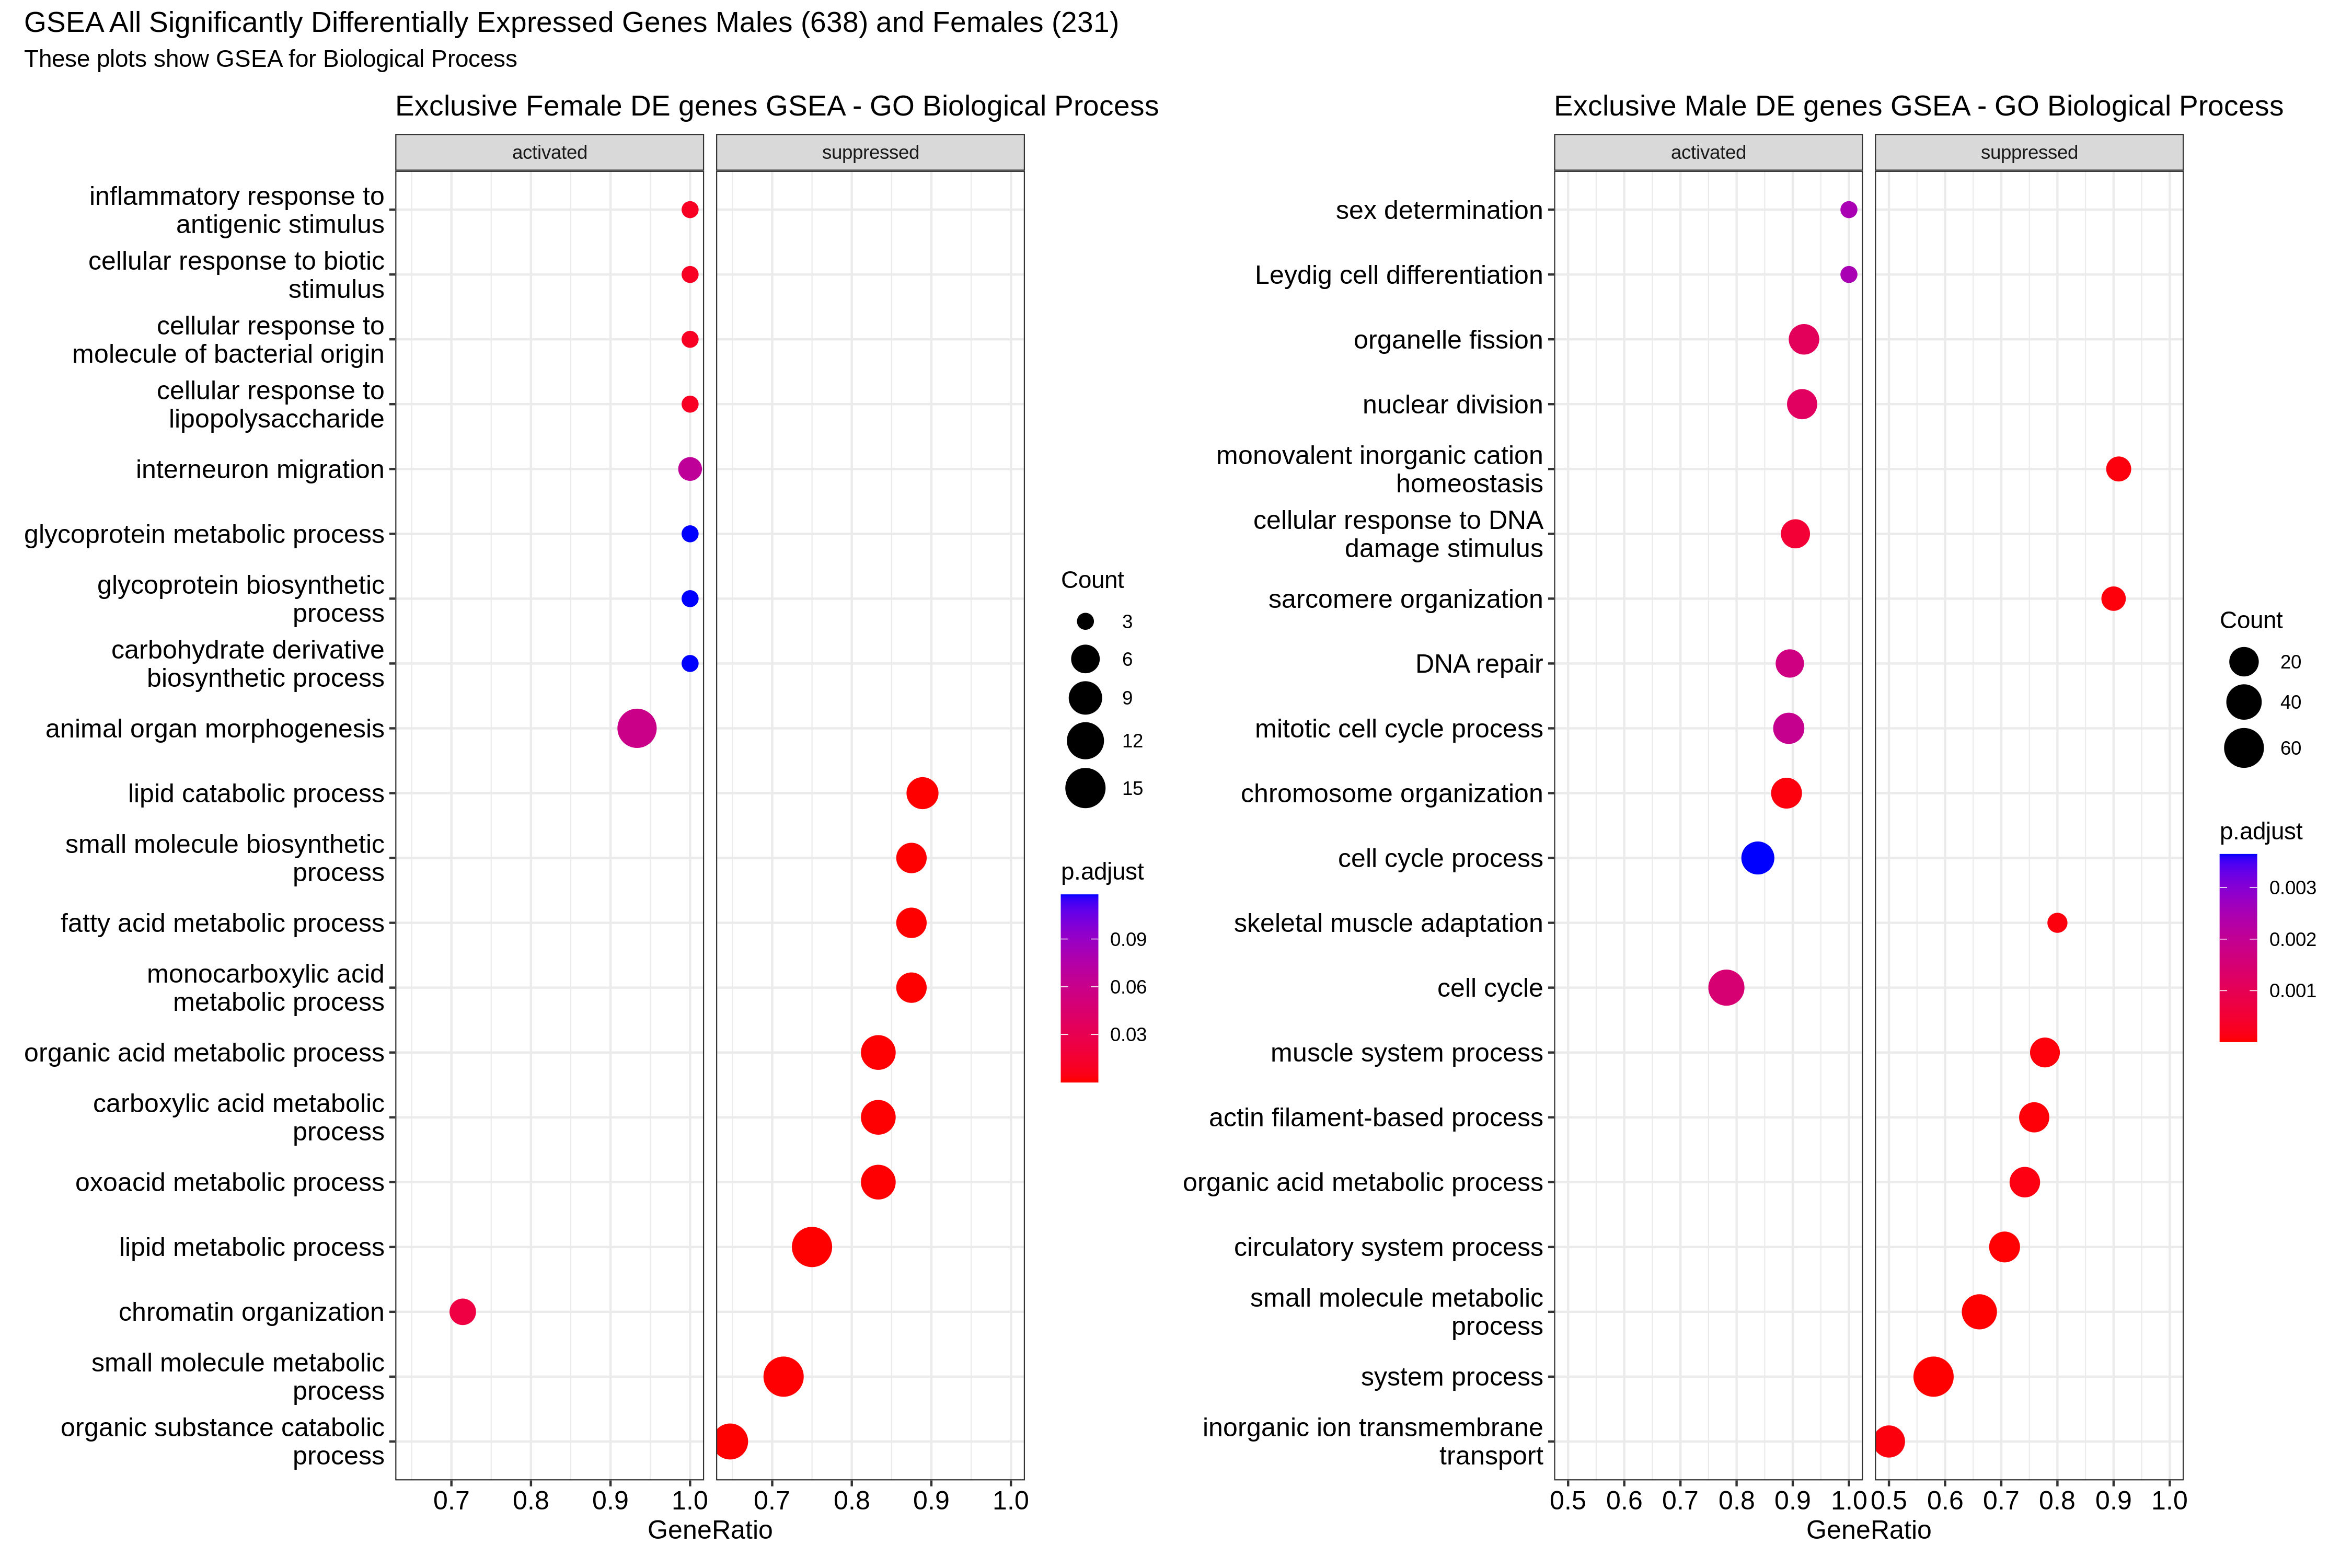
\includegraphics[width=12cm, height=8cm]{all_cancersgsea_exclusivedegenes_male_female_bp0.9.png}
	\end{frame}

	\begin{frame}
		content...
	\end{frame}

	

\end{document}
